\chapter{Experimental Analysis}\label{C11}

In this chapter, we present the experimental results of our analysis. In particular, we run all the policies considered so far in a variety of configurations and compare their performance in terms of pseudo-regret and normalized pseudo-regret. In the first section, we describe the settings of our synthetic experiments. In the second and third section we present the settings of the two real-world scenarios formalized in Chapter \ref{C10}. Then, in what follows, we show and comment the obtained results.

%Appendix: growing tmax + farsighted vs myopic + framework codice esperimenti

\begin{table}[h]
	\centering
	\caption{Experimental Analysis Summary.}
	\begin{tabular}{|c|c|c|c|c|} 
		\hhline{~----|}
		\multicolumn{1}{l|}{}     & \multicolumn{2}{c|}{{\cellcolor[rgb]{1,1,1}}\textbf{Persistency}}                               & \multicolumn{2}{c|}{{\cellcolor[rgb]{1,1,1}}\textbf{Reward}}                                 \\ 
		\hline
		\textbf{Experiment name}  & {\cellcolor[rgb]{1,1,1}}\textit{General} & {\cellcolor[rgb]{1,1,1}}\textit{Tight}   & {\cellcolor[rgb]{1,1,1}}\textit{P.R.} & {\cellcolor[rgb]{1,1,1}}\textit{N.P.R.}  \\ 
		\hline
		\textit{synthetic A,B,C}      & {\cellcolor[rgb]{1,1,1}}                 & {\cellcolor[rgb]{1,1,1}}x                               & {\cellcolor[rgb]{1,1,1}}x             & {\cellcolor[rgb]{1,1,1}}                 \\ 
		\hline
		\textit{Spotify Scenario} & {\cellcolor[rgb]{1,1,1}}x                & {\cellcolor[rgb]{1,1,1}}                                   & {\cellcolor[rgb]{1,1,1}}x             & {\cellcolor[rgb]{1,1,1}}                 \\ 
		\hline
		\textit{Rent Scenario}    & {\cellcolor[rgb]{1,1,1}}                 & {\cellcolor[rgb]{1,1,1}}x                                 & {\cellcolor[rgb]{1,1,1}}              & {\cellcolor[rgb]{1,1,1}}x                \\
		\hline
	\end{tabular}

\end{table}

\section{Synthetic Experiment Settings}
All the synthetic experiments analyzed are in \emph{tight persistency} with delay $d_{j,t}=0$ for each realization $\boldsymbol{Z_{j,t}} = (Z_{j,t,1},\dots,Z_{j,t,\Tmax})$ of the persistency vector, where each component $Z_{j,t,m}$ is a \emph{Bernoulli variable}. The feedback $R_{j, t}$ is assumed deterministic for each arm $a_j$, therefore we will omit the index $t$. $\Tmax$ is known by the learner. For each experiment we want to maximize the cumulated \emph{Pull Reward}, so we will evaluate the results in terms of \emph{Pseudo-Regret}. In this scenario, a generic realization of the persistency vector, informally called \emph{bucket}, will be a sequence of $\Tmax$ elements composed by a sub-sequence of ones followed by a sub-sequence of zeros. Note that, given a bucket $\boldsymbol{Z_{j,t}}$, since the delay $d_{j,t}$ is assumed to be 0 and we are in tight persistency, the length of the sub-sequence of ones is equal to the true length $l_{j,t}$.\\
To generate synthetic data, at each time instant t, we sample the true length $l_{j,t}$ of a new bucket $\boldsymbol{Z_{j,t}}$ from a distribution associated to the pulled arm $a_j$. More precisely, each arm $a_j$ is associated to a distribution Beta($\alpha_j$,$\beta_j$), where the parameters $\alpha_j$ and $\beta_j$ are specified according to the considered setting. The expected pull reward $\mu_j$ of an arm $a_j$ is computed in the following way:

$$\mu_j = R_j\sum_{i=1}^{\Tmax}i\bigg(F_j\bigg(\frac{i}{\Tmax}\bigg)-F_j\bigg(\frac{i-1}{\Tmax}\bigg)\bigg) \ ,$$
where $F_j$ is the cumulative distribution function of the Beta($\alpha_j$,$\beta_j$).
Below we present three significant settings analyzed: \emph{Synthetic A}, \emph{Synthetic B}, \emph{Synthetic C}.

\begin{figure}[t]
	\centering
	\begin{tabular}{llllllllll}
		\cline{2-9}
		\multicolumn{1}{l|}{} & \multicolumn{1}{l|}{1} & \multicolumn{1}{l|}{1} & \multicolumn{1}{l|}{1} & \multicolumn{1}{l|}{1} & \multicolumn{1}{l|}{1} & \multicolumn{1}{l|}{0} & \multicolumn{1}{l|}{0} & \multicolumn{1}{l|}{0} &  \\ \cline{2-9}
		& \textit{1}             & \textit{}              &                        &                        &                        &                        & \multicolumn{3}{c}{\textit{ $\Tmax$}}                 
	\end{tabular}
	\caption{Example of bucket in synthetic setting. In this example $\Tmax=8$, the legth of the vector. The first 5 components are successes (1), meaning that the true length of the vector is $l=5$.}
	\label{sbucket}
\end{figure}
%A lot of real problems can be easily represented in this way, furthermore, here we focus our attention on this scenario as it directly attacks the problem treated, givining a basic answer to the question we asked ourselves: "What happens if the reward is not a scalar but is persistent over time?"
\subsection{Synthetic A}\label{SA}
In this setting, the true length $l_{j,t}$ is sampled from a Beta distribution with parameters $a_j = b_j = 1$, for each arm $a_j$, for each time instant t. In this configuration the Beta distribution is equivalent to the uniform distribution. The feedback $R_j$ is set incrementally for each arm $a_j$. Here the best arm is the one with maximum feedback $R_j$. In fact, the magnitude of $R_j$ does not influence the true length $l_{j,t}$ which is generated uniformly at random.  We set $\Tmax = 50$. The experiment is repeated for 50 independent runs. The full description of the arms is provided in Table \ref{tabSA}.



\begin{table}[H]
	
	\centering	
	\caption{Description of the arms in setting Synthetic A.}
	\begin{tabular}{|c|cccccccccc|}
		\hline
		\textbf{Arm}       & $a_0$ & $a_1$ & $a_2$ & $a_3$ & $a_4$ & $a_5$ & $a_6$ & $a_7$ & $a_8$ & $a_9$ \\ \hline
		\textbf{R}         & 1     & 2     & 3     & 4     & 5     & 6     & 7     & 8     & 9     & 10    \\
		$\boldsymbol{\mu}$ & 25.5  & 51    & 76.5  & 102   & 127.5 & 153   & 178.5 & 204   & 229.5 & 255   \\ \hline
	\end{tabular}
	
\label{tabSA}
\end{table}
\subsection{Synthetic B}\label{SB}
In this setting, for each time instant t, the true length $l_{j,t}$ is sampled from a Beta distribution depending on the pulled arm $a_j$. For each arm $a_j$, the feedback is $R_j=1$. This implies that the best arm is the one which is associated to the Beta with the highest mean. We set $\Tmax=50$. The experiment is repeated for 50 independent runs. The full description of the arms is provided in Table \ref{tabSB}.


\begin{table}[H]
	\centering
	\caption{Description of the arms in setting Synthetic B.}
	
	\begin{tabular}{|c|cccccc|}
		\hline
		\textbf{Arm}          & $a_0$ & $a_1$ & $a_2$ & $a_3$ & $a_4$ & $a_5$ \\ \hline
		\textbf{R}            & 1     & 1     & 1     & 1     & 1     & 1     \\
		$\boldsymbol{\alpha}$ & 2     & 4     & 6     & 8     & 10    & 12    \\
		$\boldsymbol{\beta}$  & 8     & 8     & 8     & 8     & 8     & 8     \\
		$\boldsymbol{\mu}$    & 10.50 & 17.17 & 21.93 & 25.50 & 28.28 & 30.3  \\ \hline
	\end{tabular}

\label{tabSB}
\end{table}
\begin{figure}[H]
	\centering
	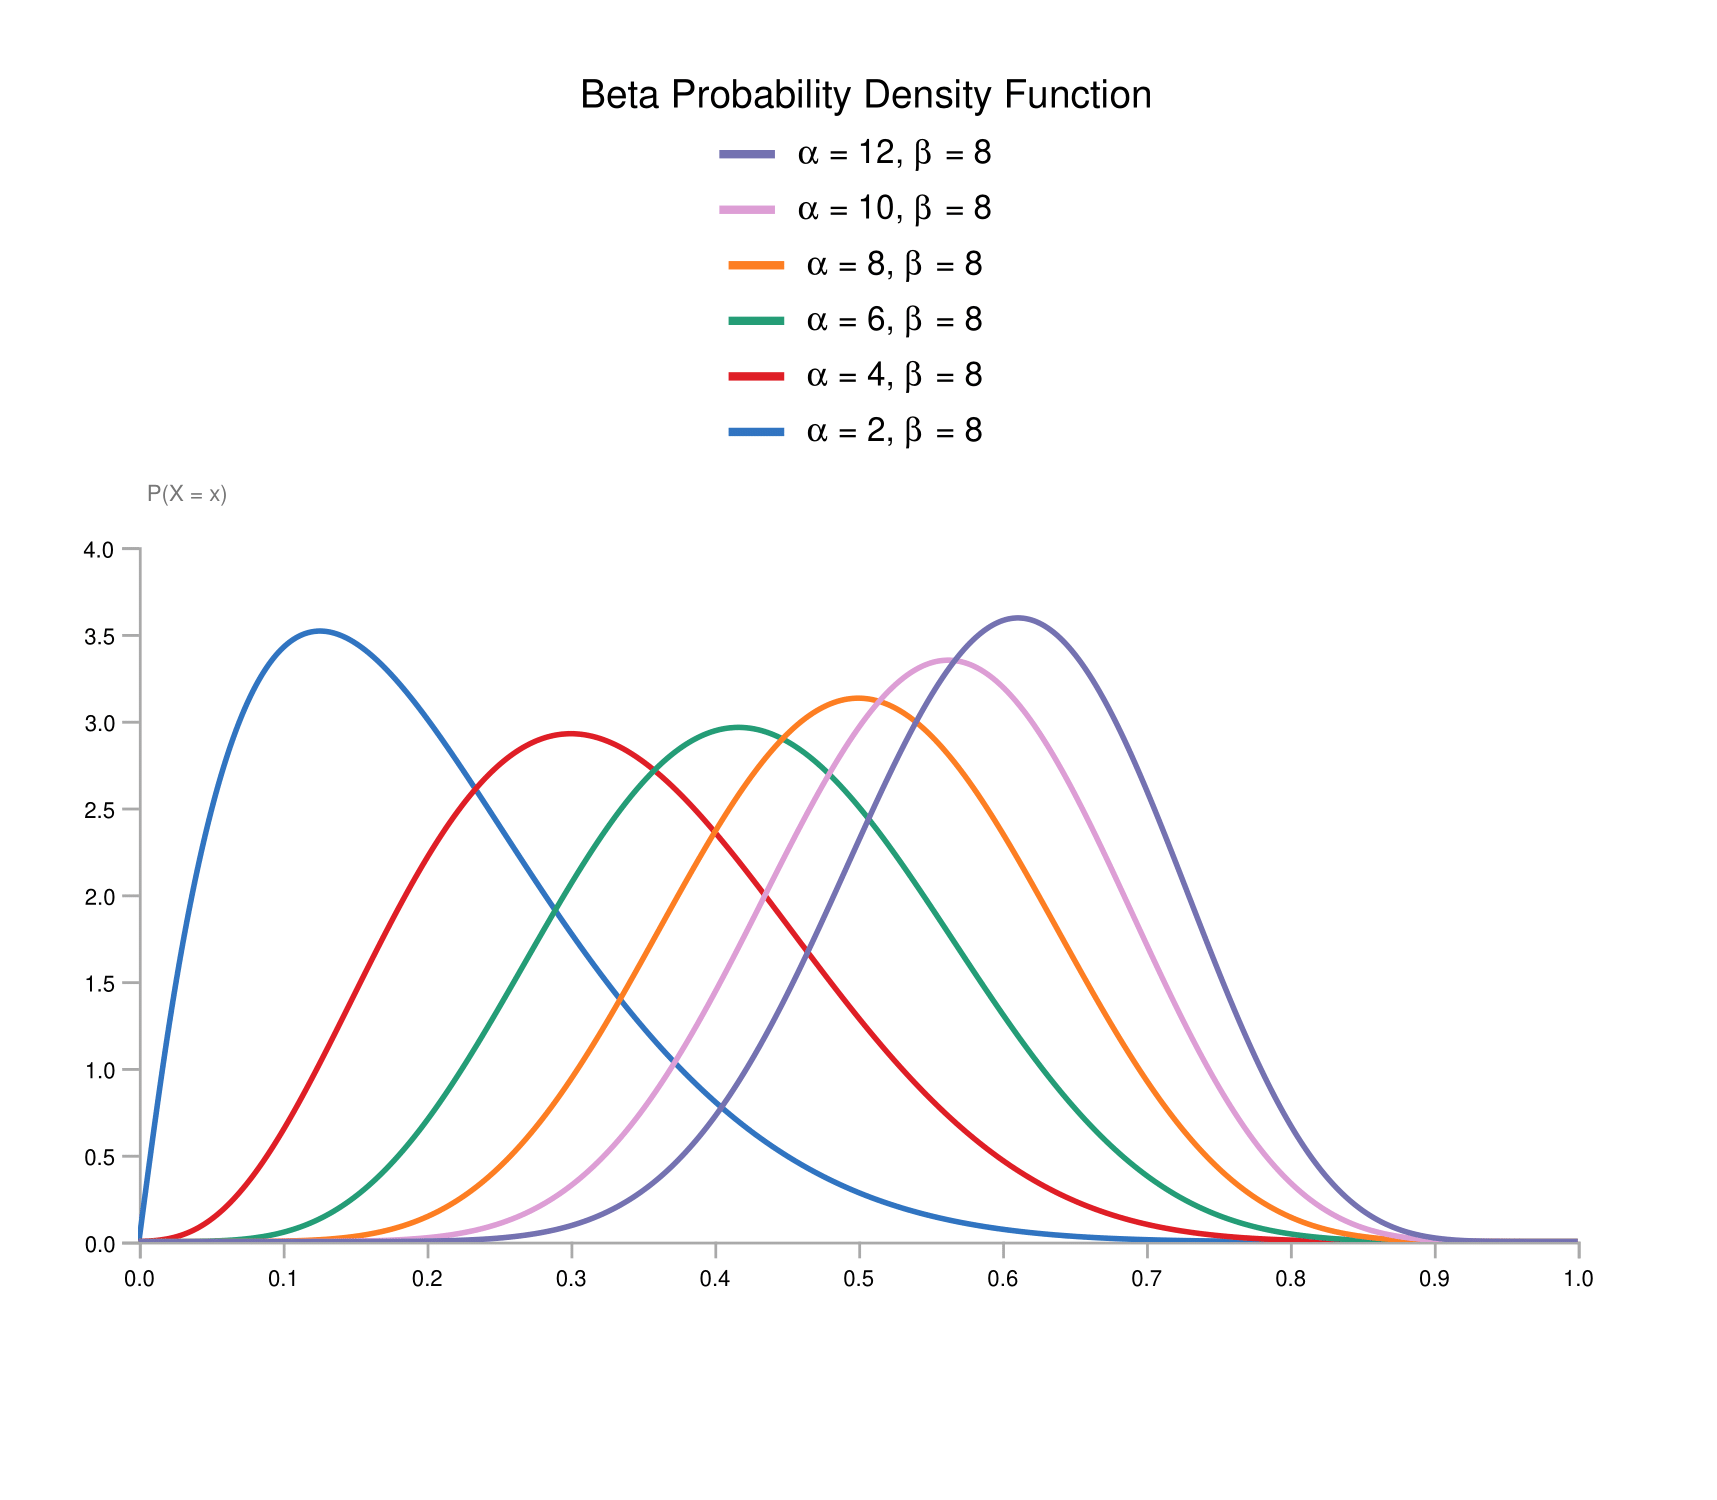
\includegraphics[width=6.26cm]{./images/chart (1)-1.png}\quad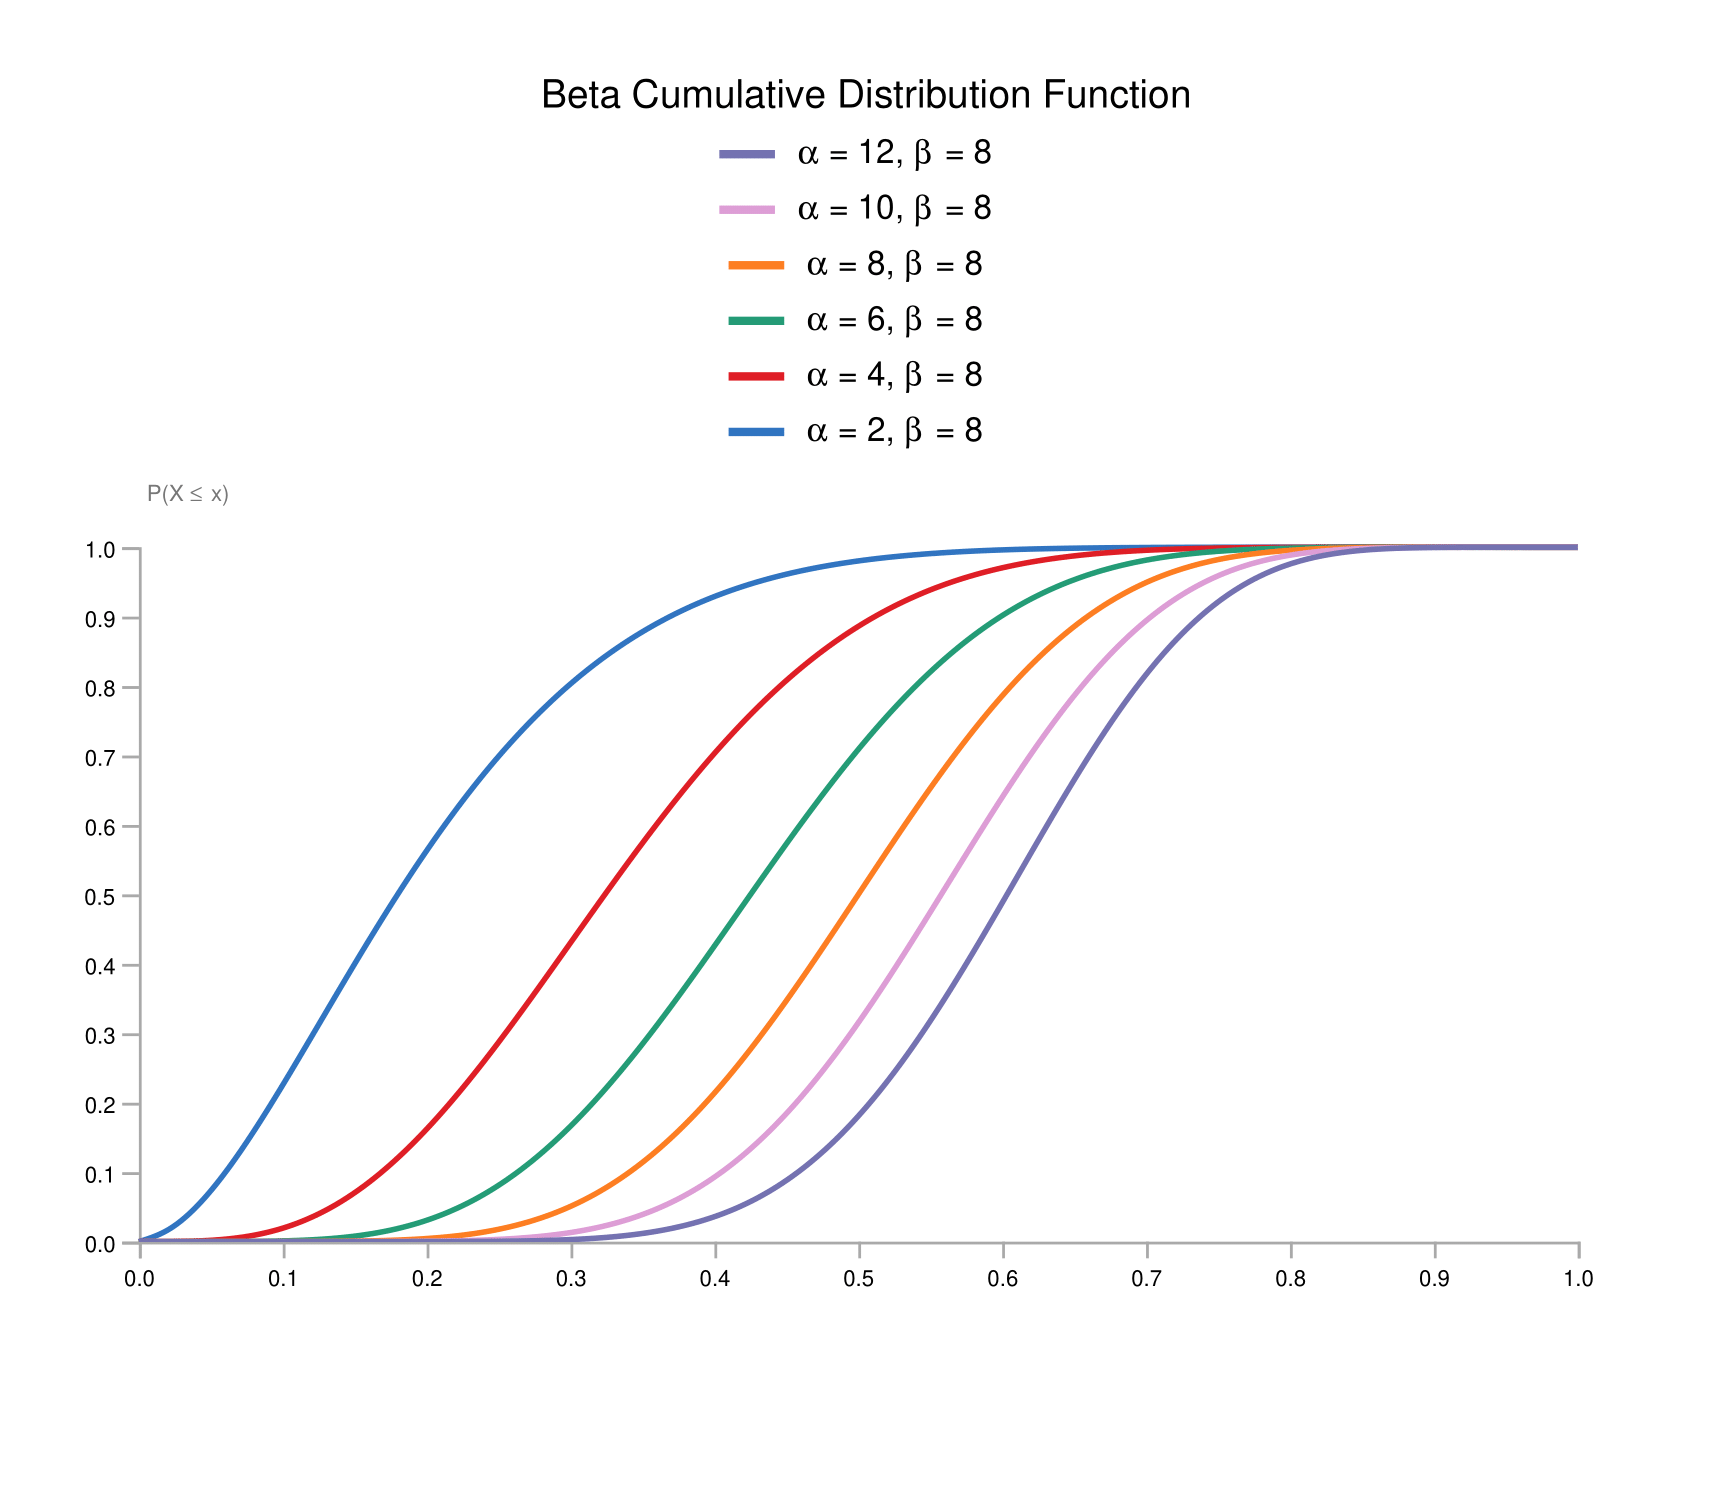
\includegraphics[width=6cm]{./images/chart (2)-1.png}
	\caption{Probability density function and cumulative distribution function of the Beta distributions considered in settings Synthetic B and Synthetic C.}
	\label{beta}
\end{figure}

\subsection{Synthetic C}\label{SC}

In this setting, we model the common situation where high feedback discourage long persistency, as previously discussed in Chapter \ref{CF}. At each time t, the true length $l_{j,t}$ is sampled from a Beta distribution depending on the pulled arm $a_j$. For each arm $a_j$, the feedback is $R_j$ is set such that to higher Beta mean corresponds lower feedback. We set $\Tmax=50,100,150,200$. For each $\Tmax$ adopted, the experiment is repeated for 50 independent runs. The full description of the arms is provided in Table \ref{tabSC} where with $\mu_{\Tmax}$ we indicate the expected pull reward in the configuration where $\Tmax$ is adopted.



\begin{table}[H]
	\centering
	\caption{Description of the arms in setting Synthetic C.}
	
	\begin{tabular}{|c|cccccc|}
		\hline
		\textbf{Arm}          & $a_0$ & $a_1$ & $a_2$ & $a_3$ & $a_4$ & $a_5$ \\ \hline
		\textbf{R}            & 6     & 5     & 4     & 3     & 2     & 1     \\
		$\boldsymbol{\alpha}$ & 2     & 4     & 6     & 8     & 10    & 12    \\
		$\boldsymbol{\beta}$  & 8     & 8     & 8     & 8     & 8     & 8     \\
		$\boldsymbol{\mu_{50}}$    & 63.00 & 85.83 & 87.71 & 76.50 & 56.55 & 30.50  \\ 
		$\boldsymbol{\mu_{100}}$    & 123.00 & 169.16 & 173.43 & 151.50 & 112.11 & 60.50  \\ 
		$\boldsymbol{\mu_{150}}$    & 183.00 & 252.50 & 259.14 & 226.50 & 167.67 & 90.5  \\ 
		$\boldsymbol{\mu_{200}}$    & 243.00 & 335.83 & 344.85 & 301.50 & 223.22 & 120.50  \\ \hline
	\end{tabular}
	
	\label{tabSC}
\end{table}

%\section{The Spotify Playlist Problem Setting}
%
%\section{The Rental Pricing Problem Setting}



\section{Results}

\begin{figure}[H]
	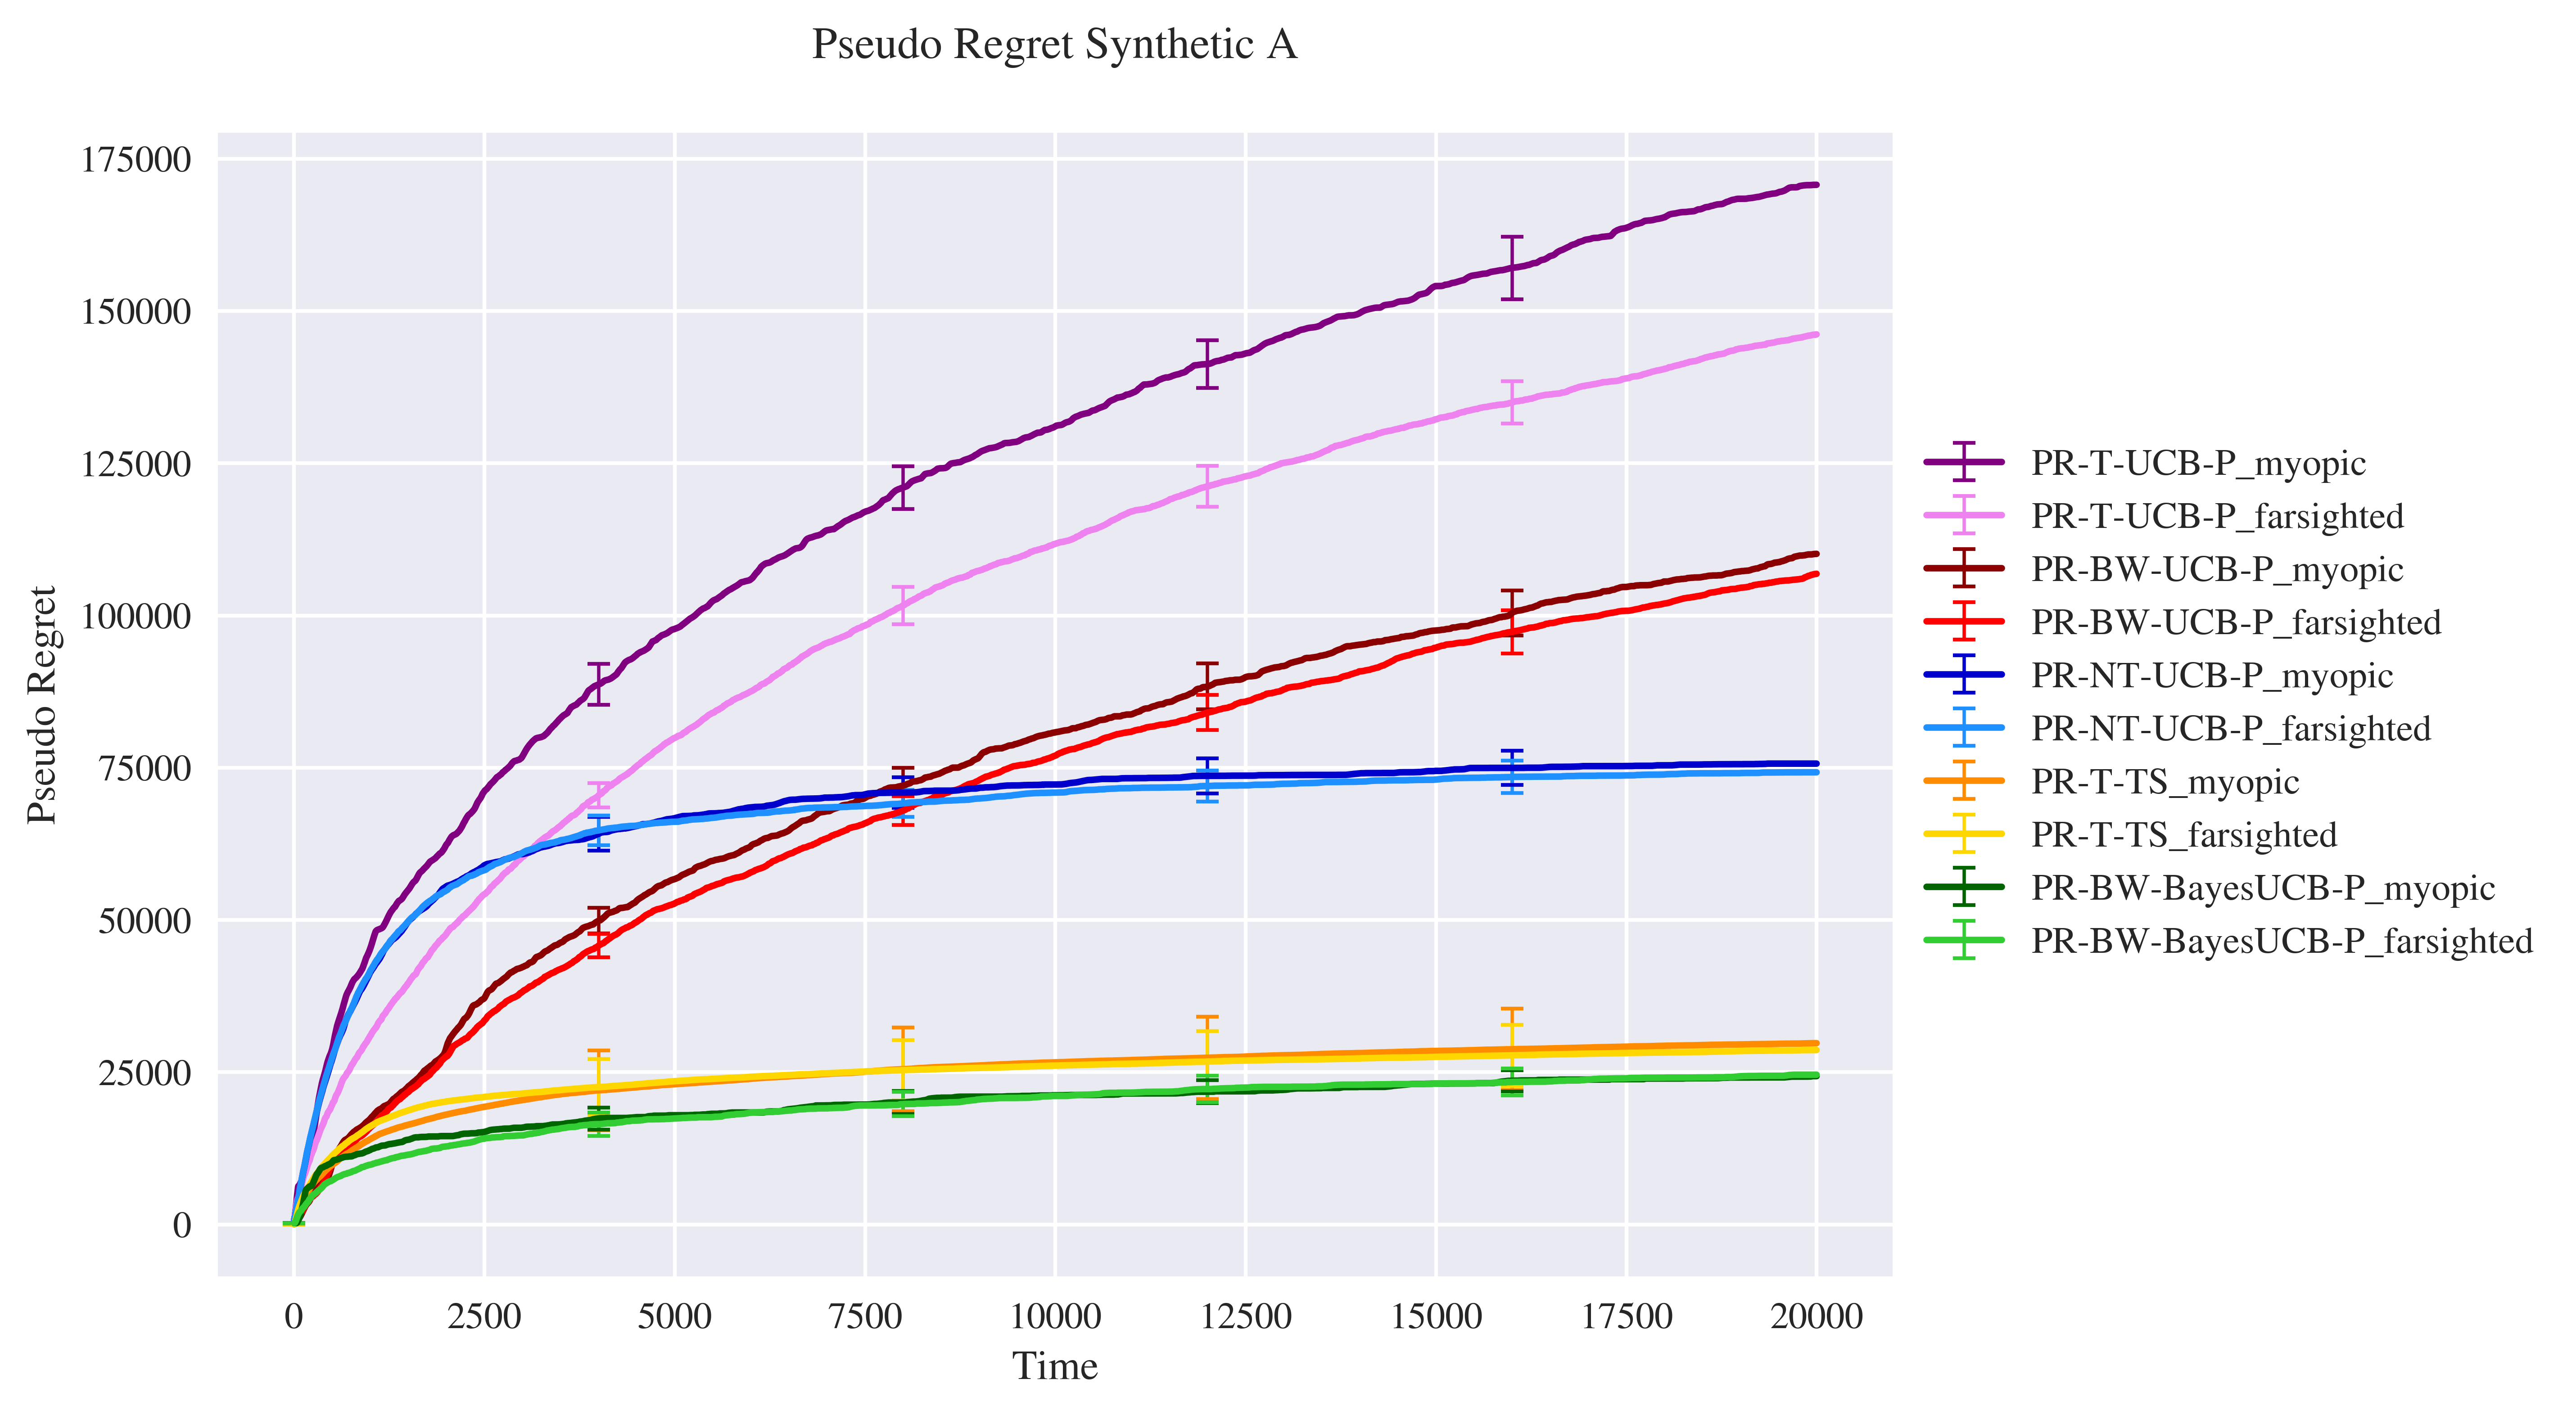
\includegraphics[width=16cm]{./images/ANALYTICS/experiment_A ANALYTICS.png}
	\centering	
	\caption{Pseudo regret plot of the experiment Synthetic A.}
	\label{f:a}
\end{figure}
\begin{figure}[H]
	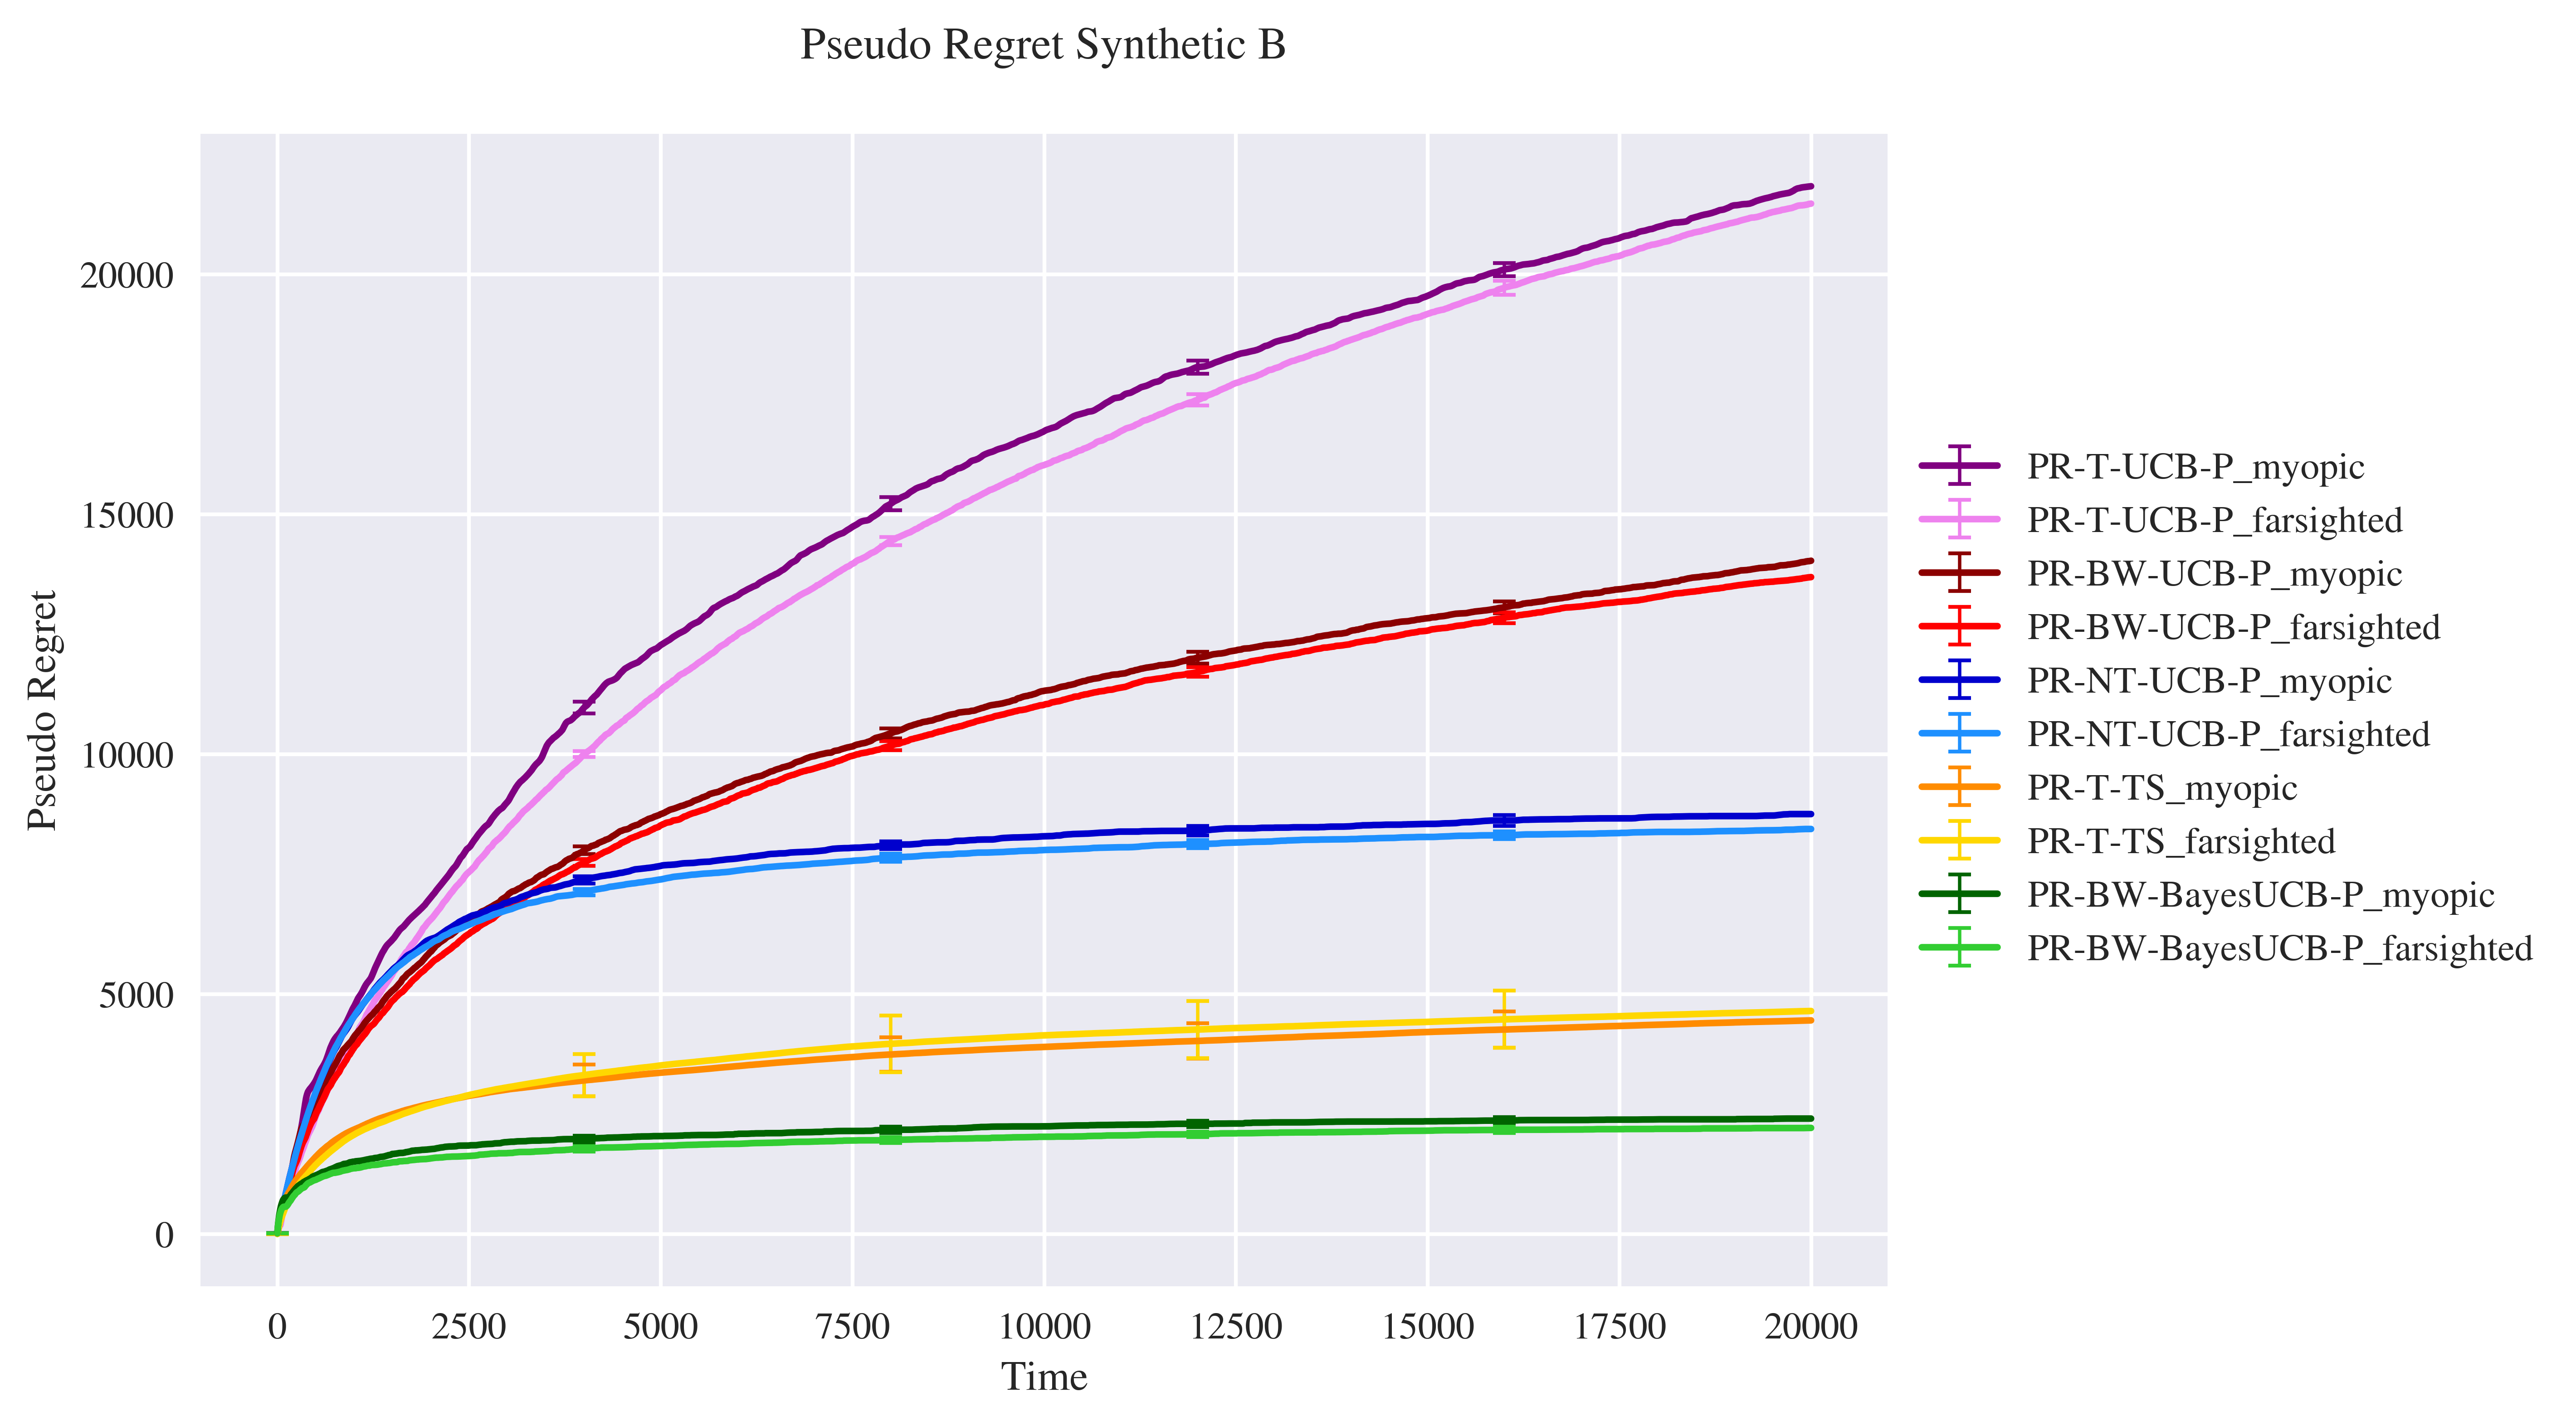
\includegraphics[width=16cm]{./images/ANALYTICS/experiment_B ANALYTICS.png}
	\centering	
	\caption{Pseudo regret plot of the experiment Synthetic B. }
	\label{f:b}
\end{figure}

\begin{figure}[H]
	
	\centering
	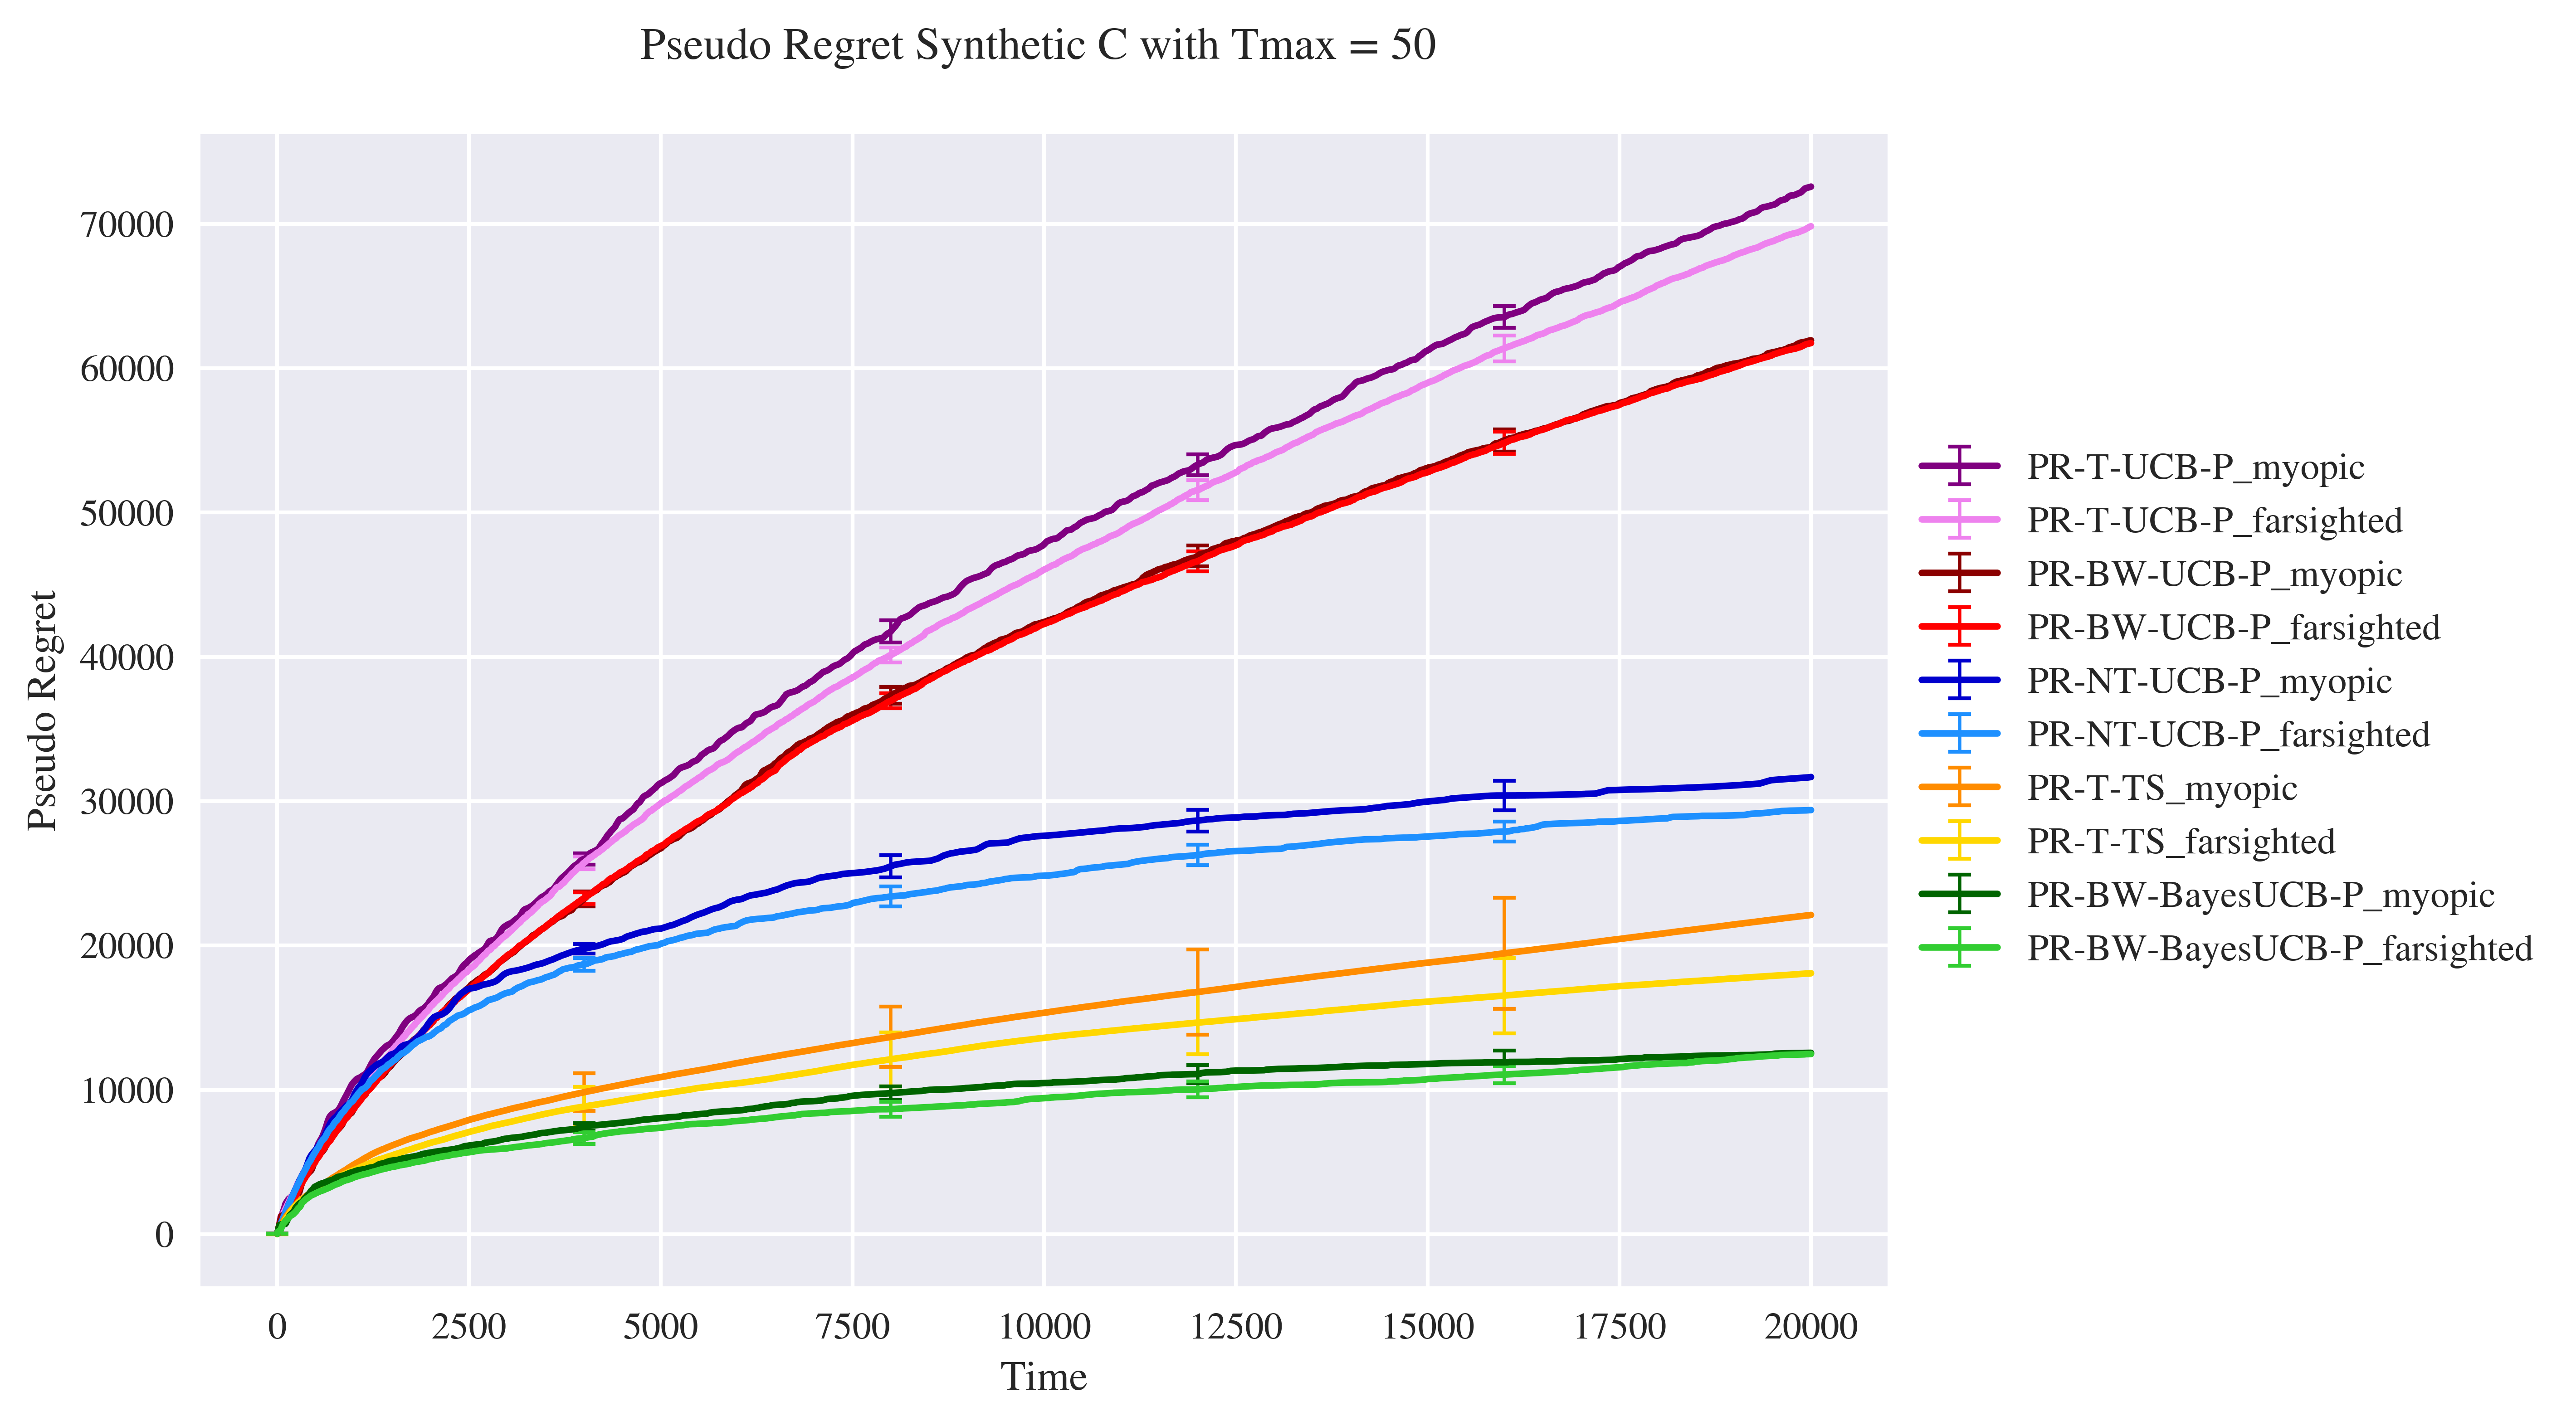
\includegraphics[width=9.5cm]{./images/ANALYTICS/experiment_C_50 ANALYTICS.png}\quad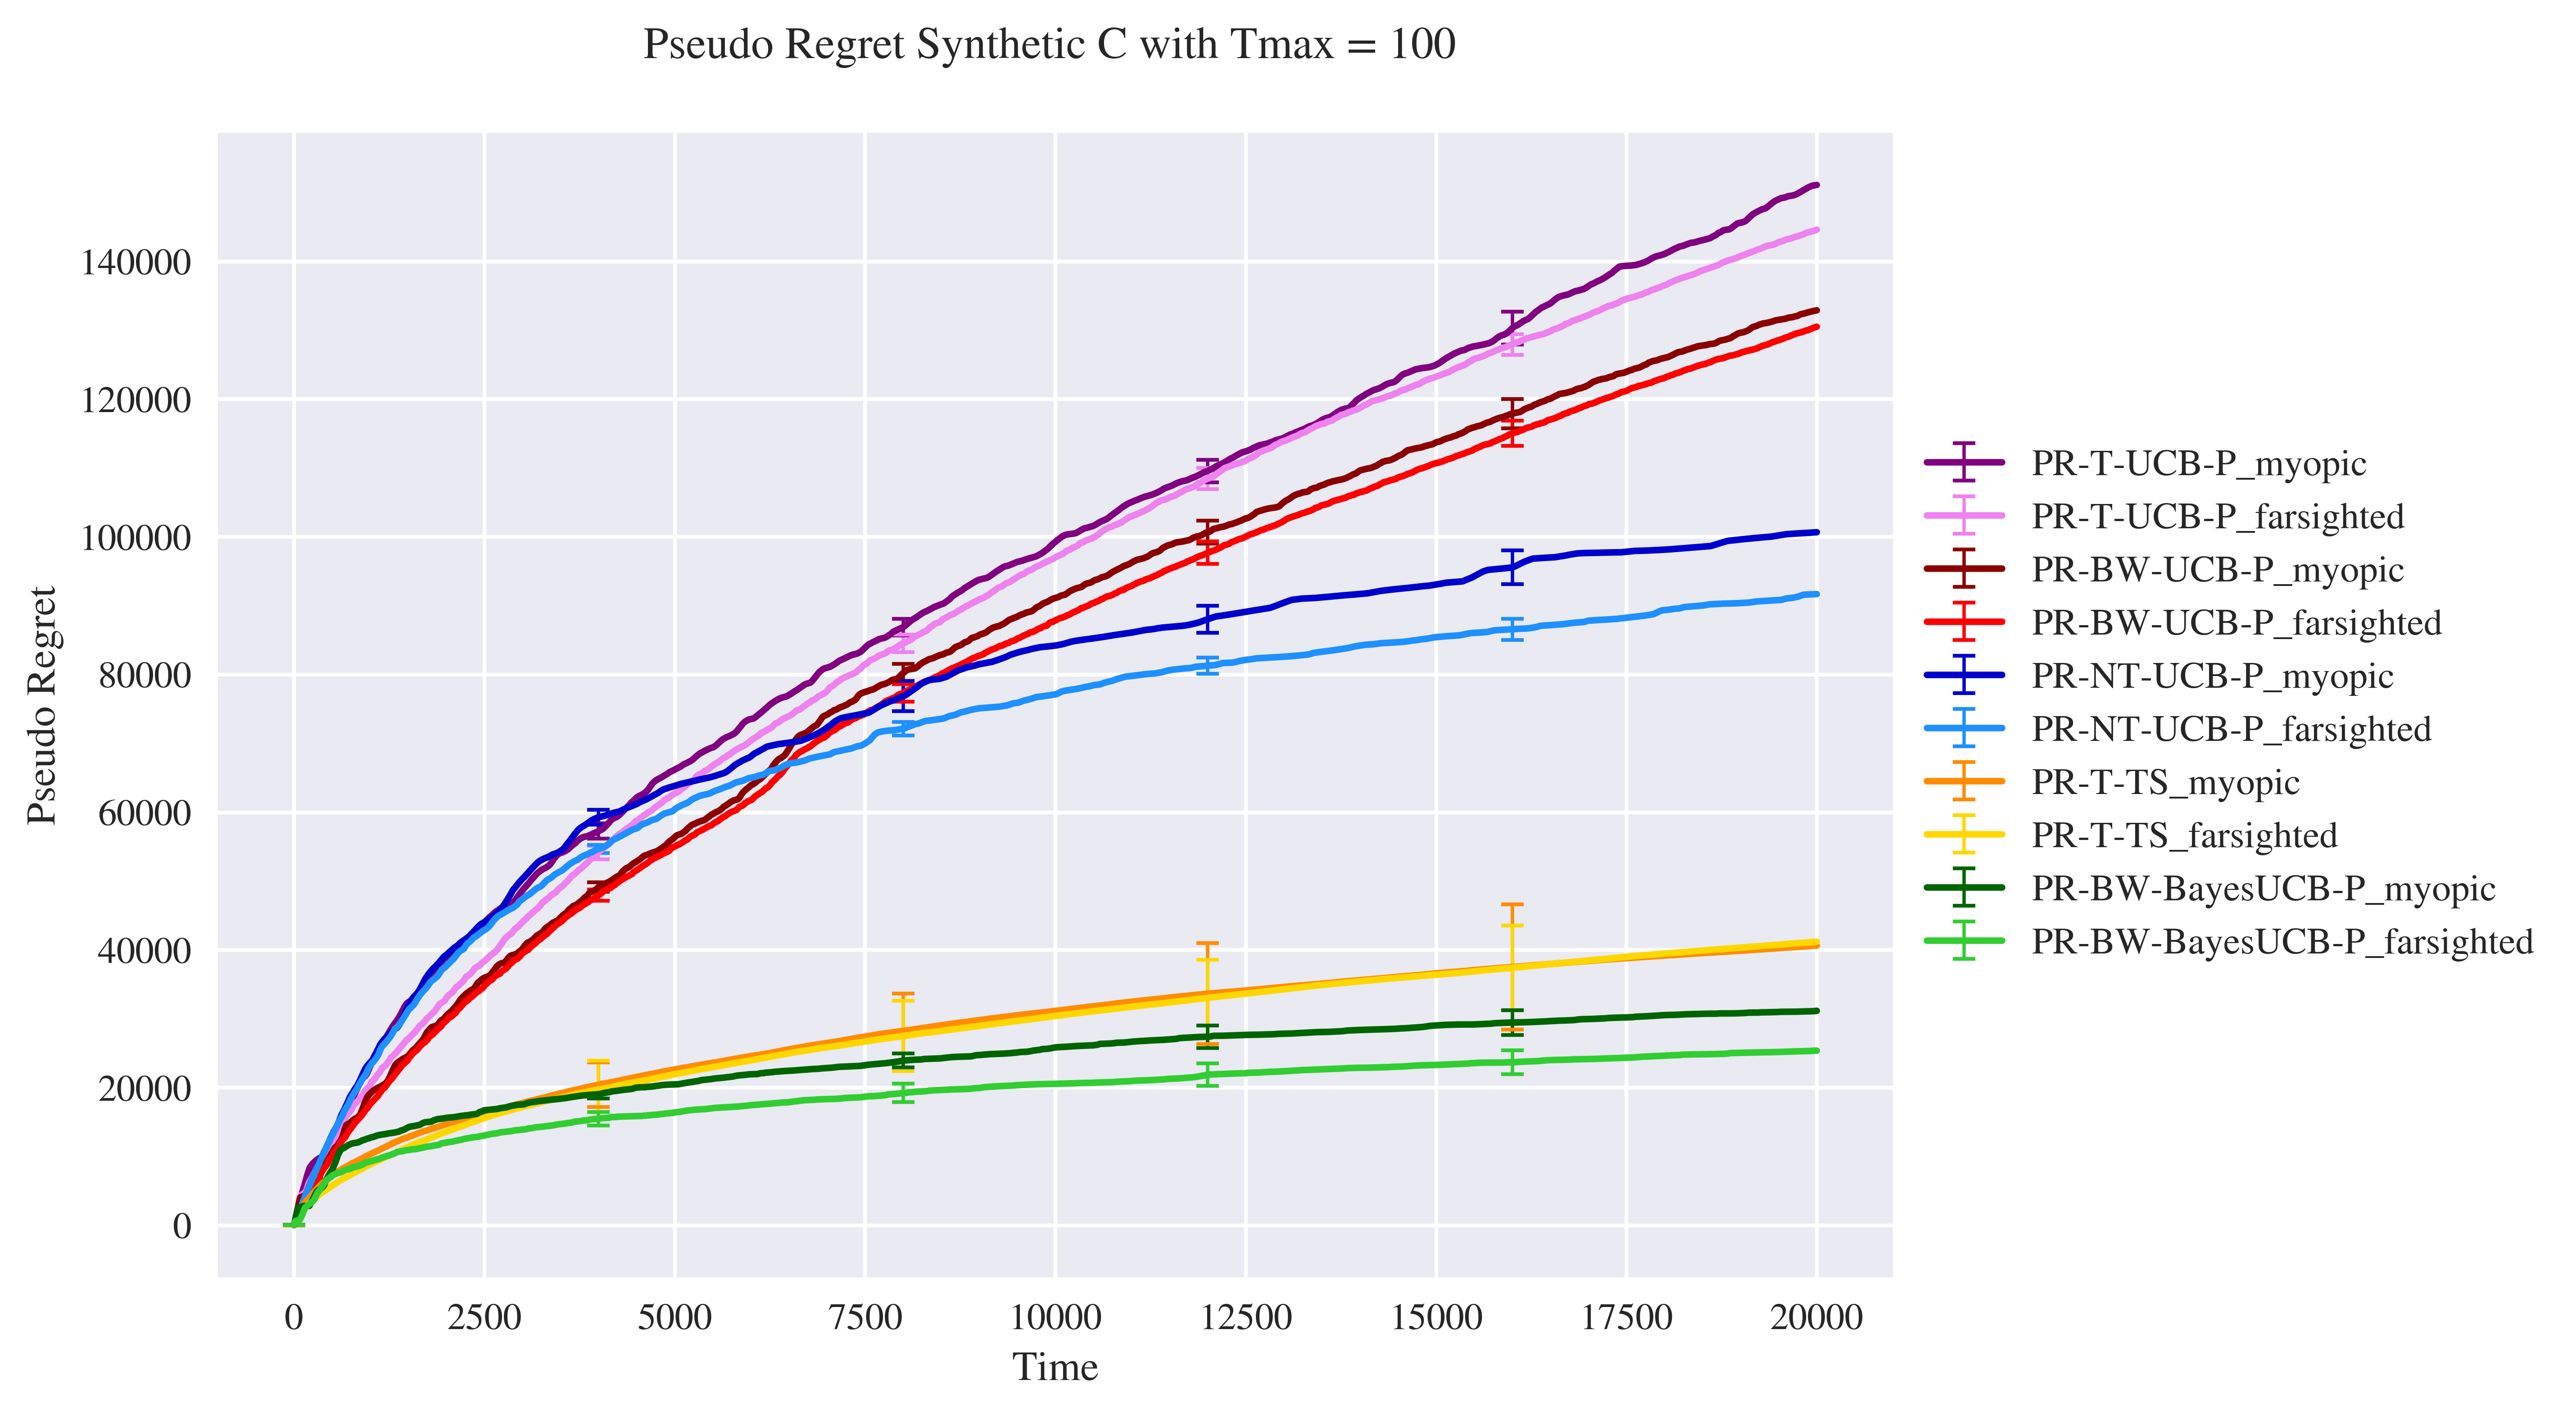
\includegraphics[width=9.5cm]{./images/ANALYTICS/experiment_C_100 ANALYTICS.png}
	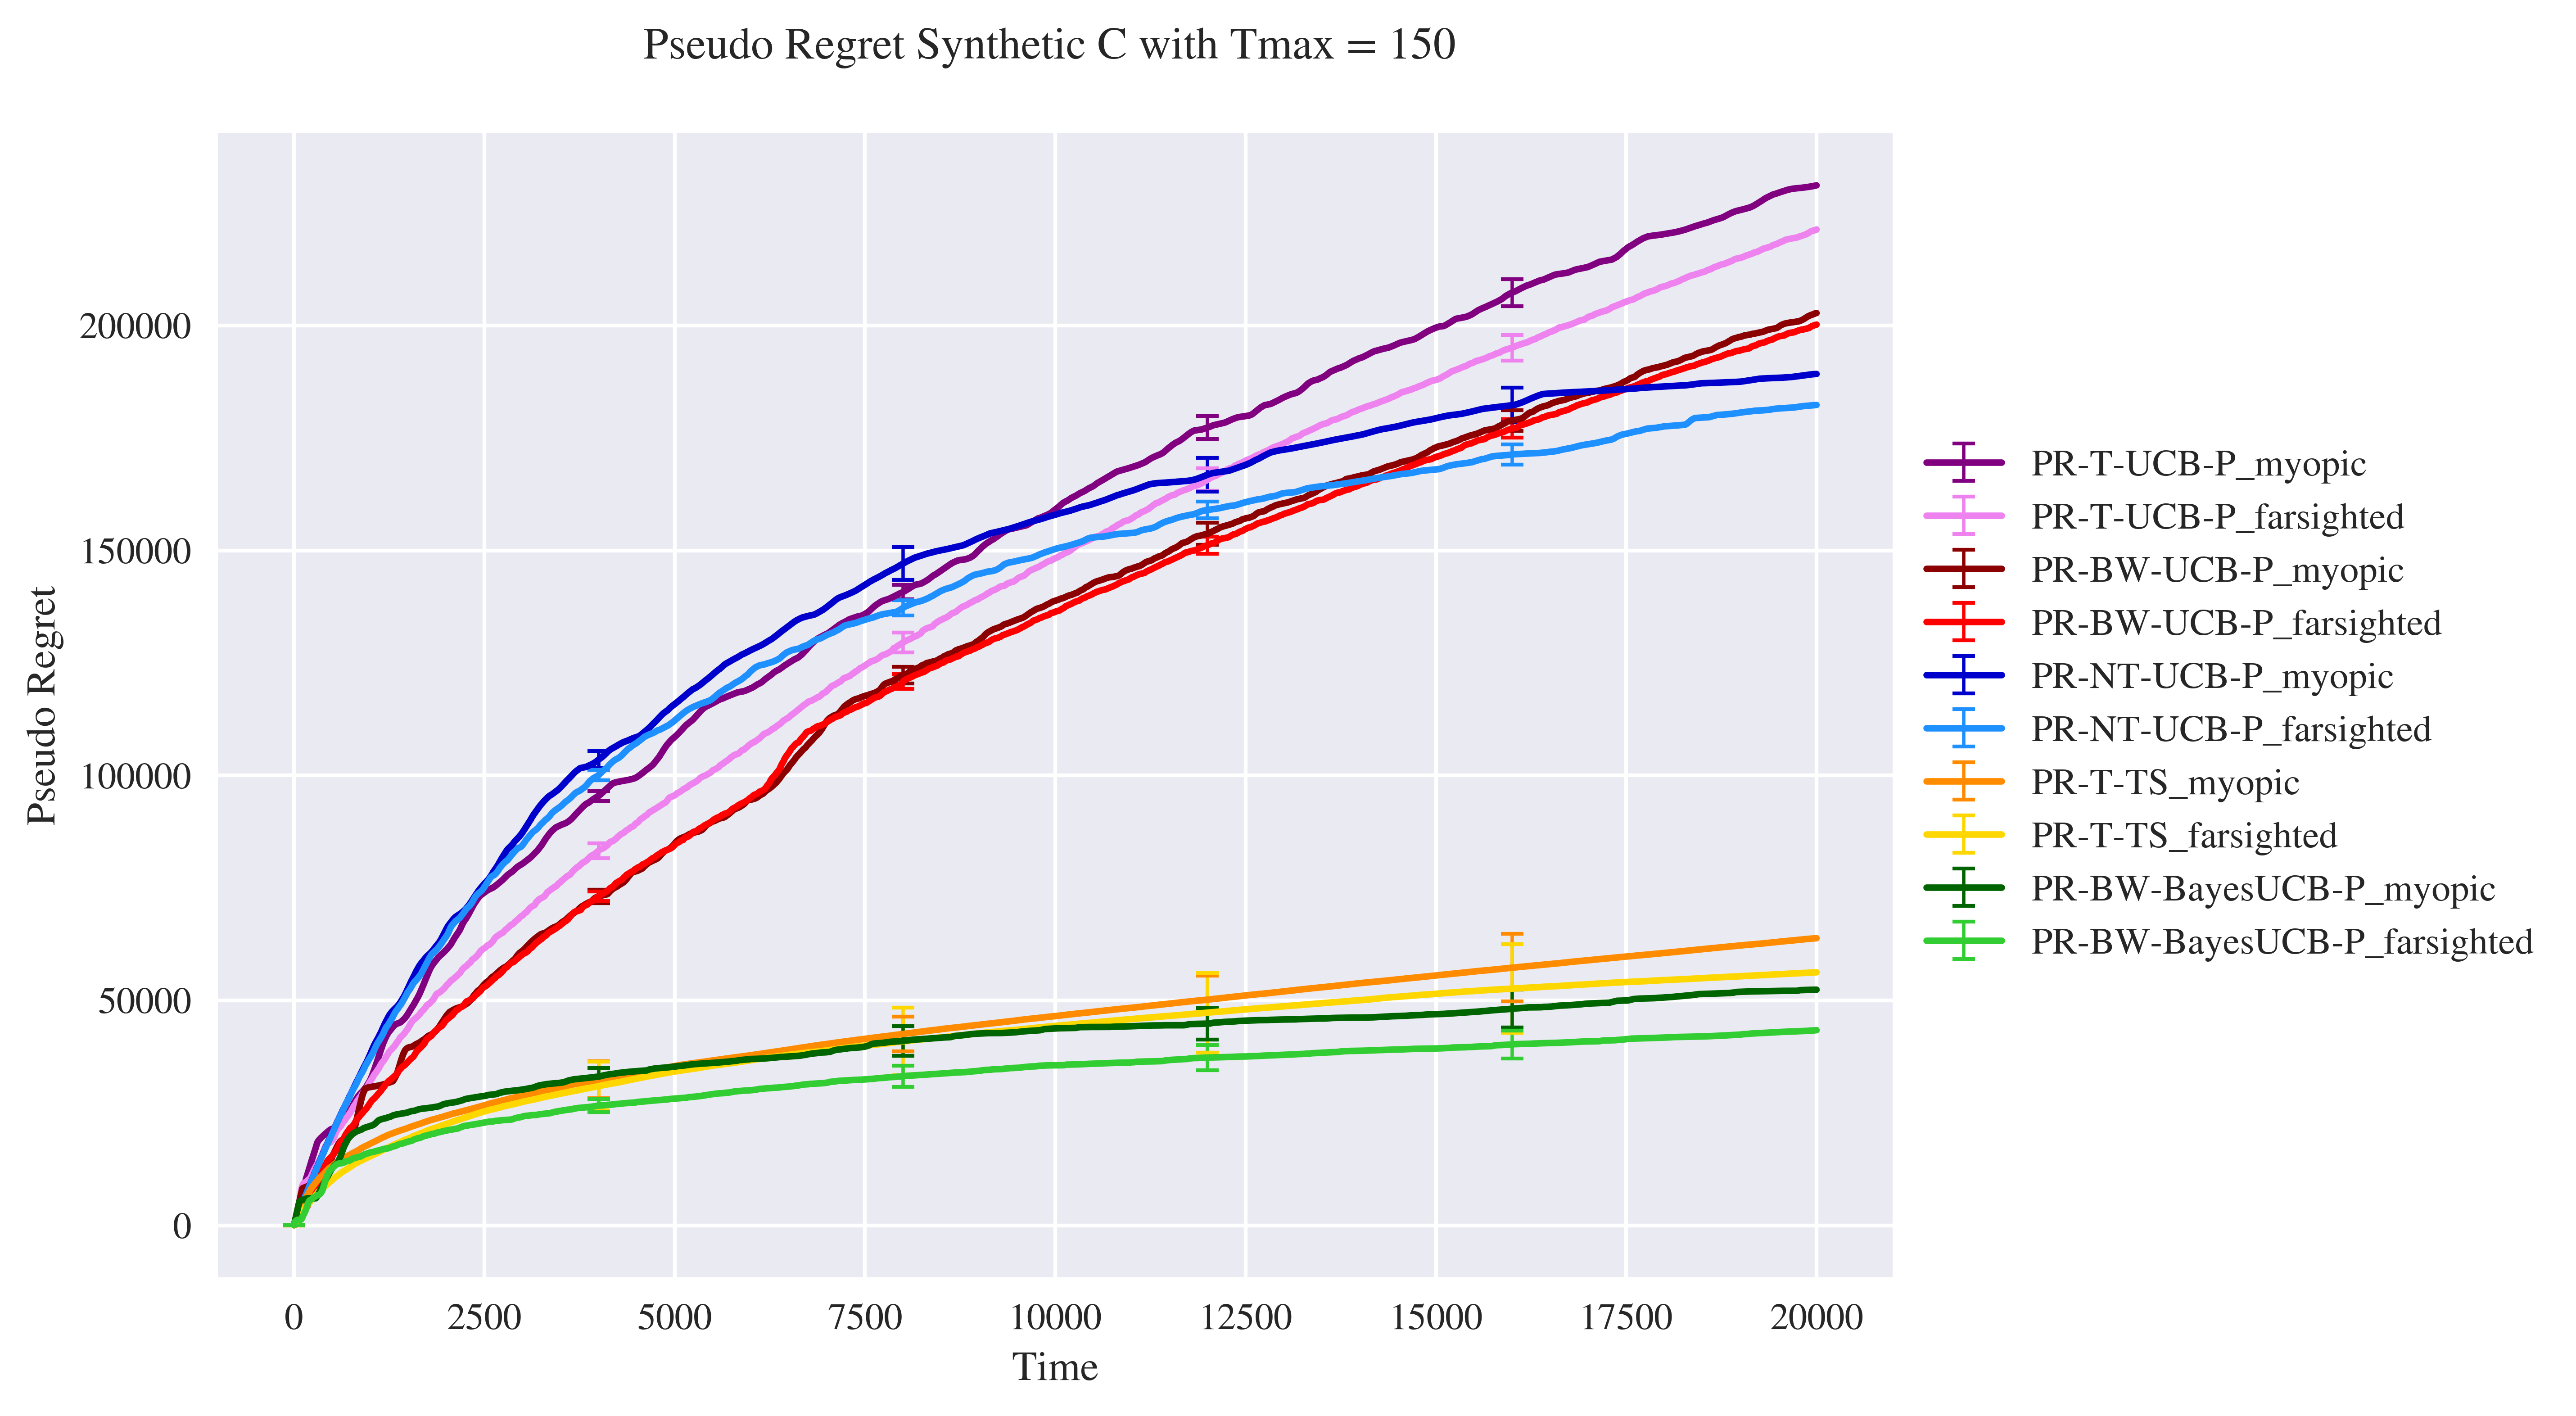
\includegraphics[width=9.5cm]{./images/ANALYTICS/experiment_C_150 ANALYTICS.png}\quad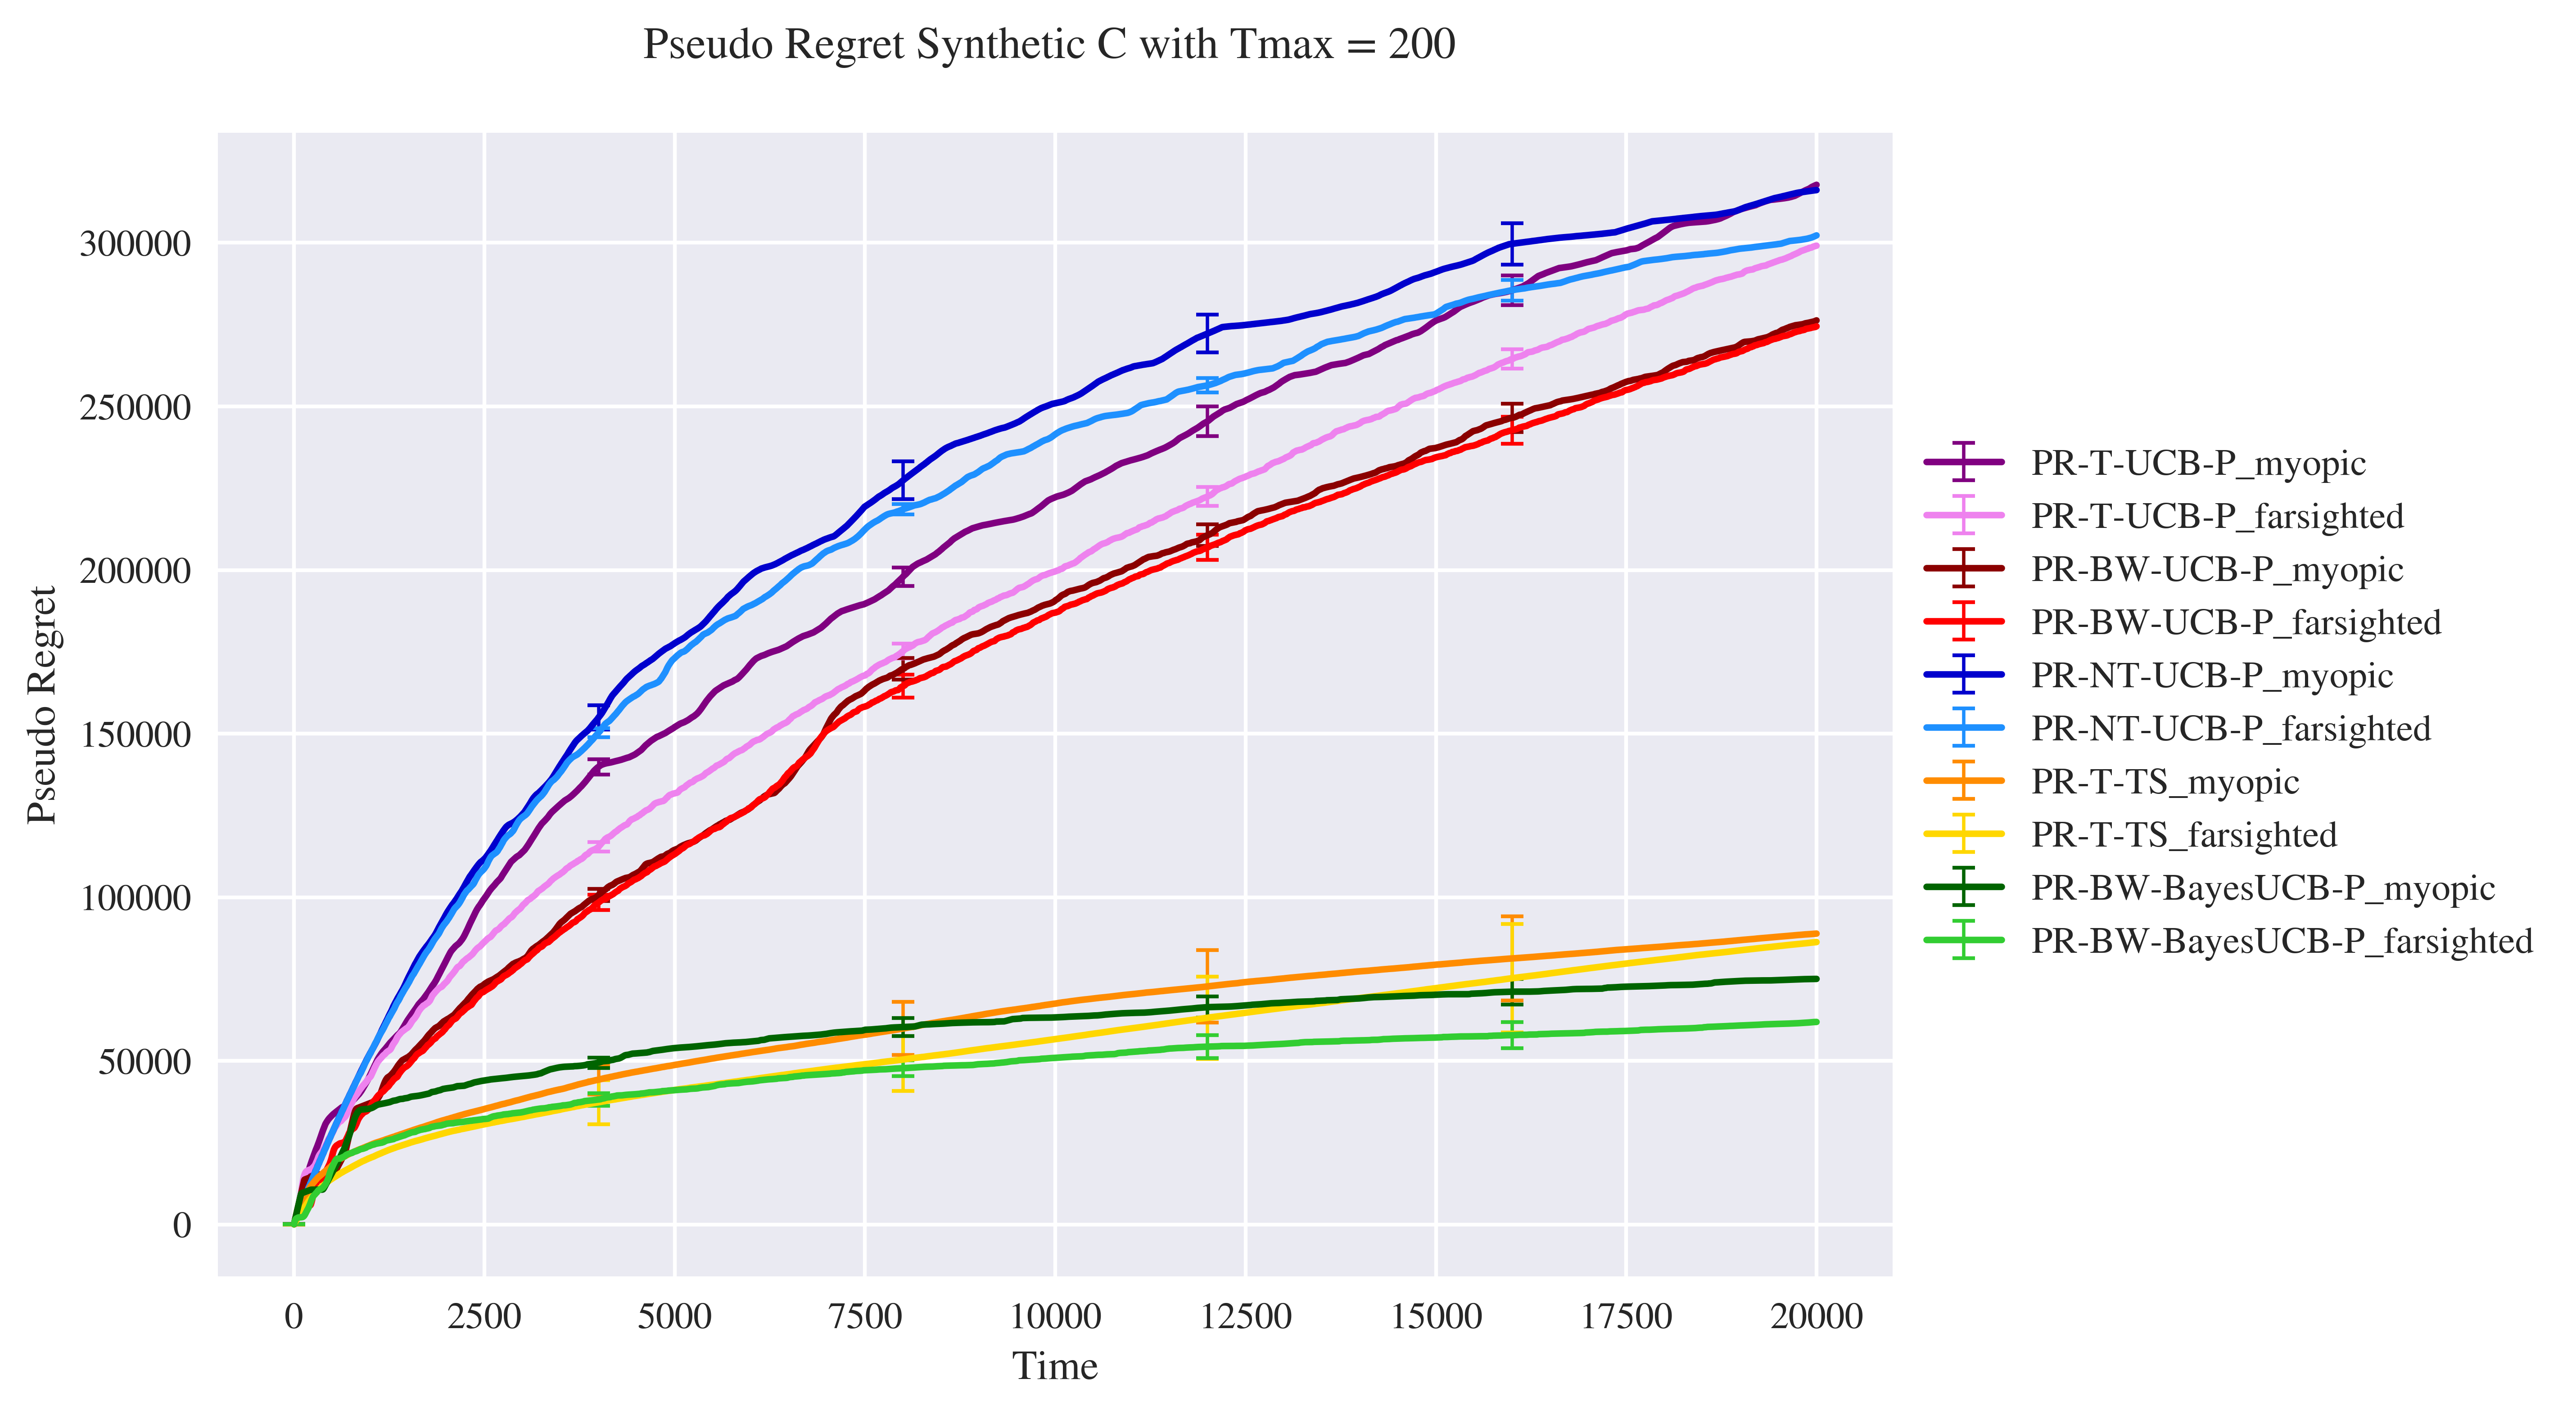
\includegraphics[width=9.5cm]{./images/ANALYTICS/experiment_C_200 ANALYTICS.png}
	\caption{Pseudo regret plots of the experiment Synthetic C. From the top: $\Tmax = 50, 100, 150, 200$.}
	\label{f:c}
	
\end{figure}

%SPOTIFY

\begin{figure}[H]
		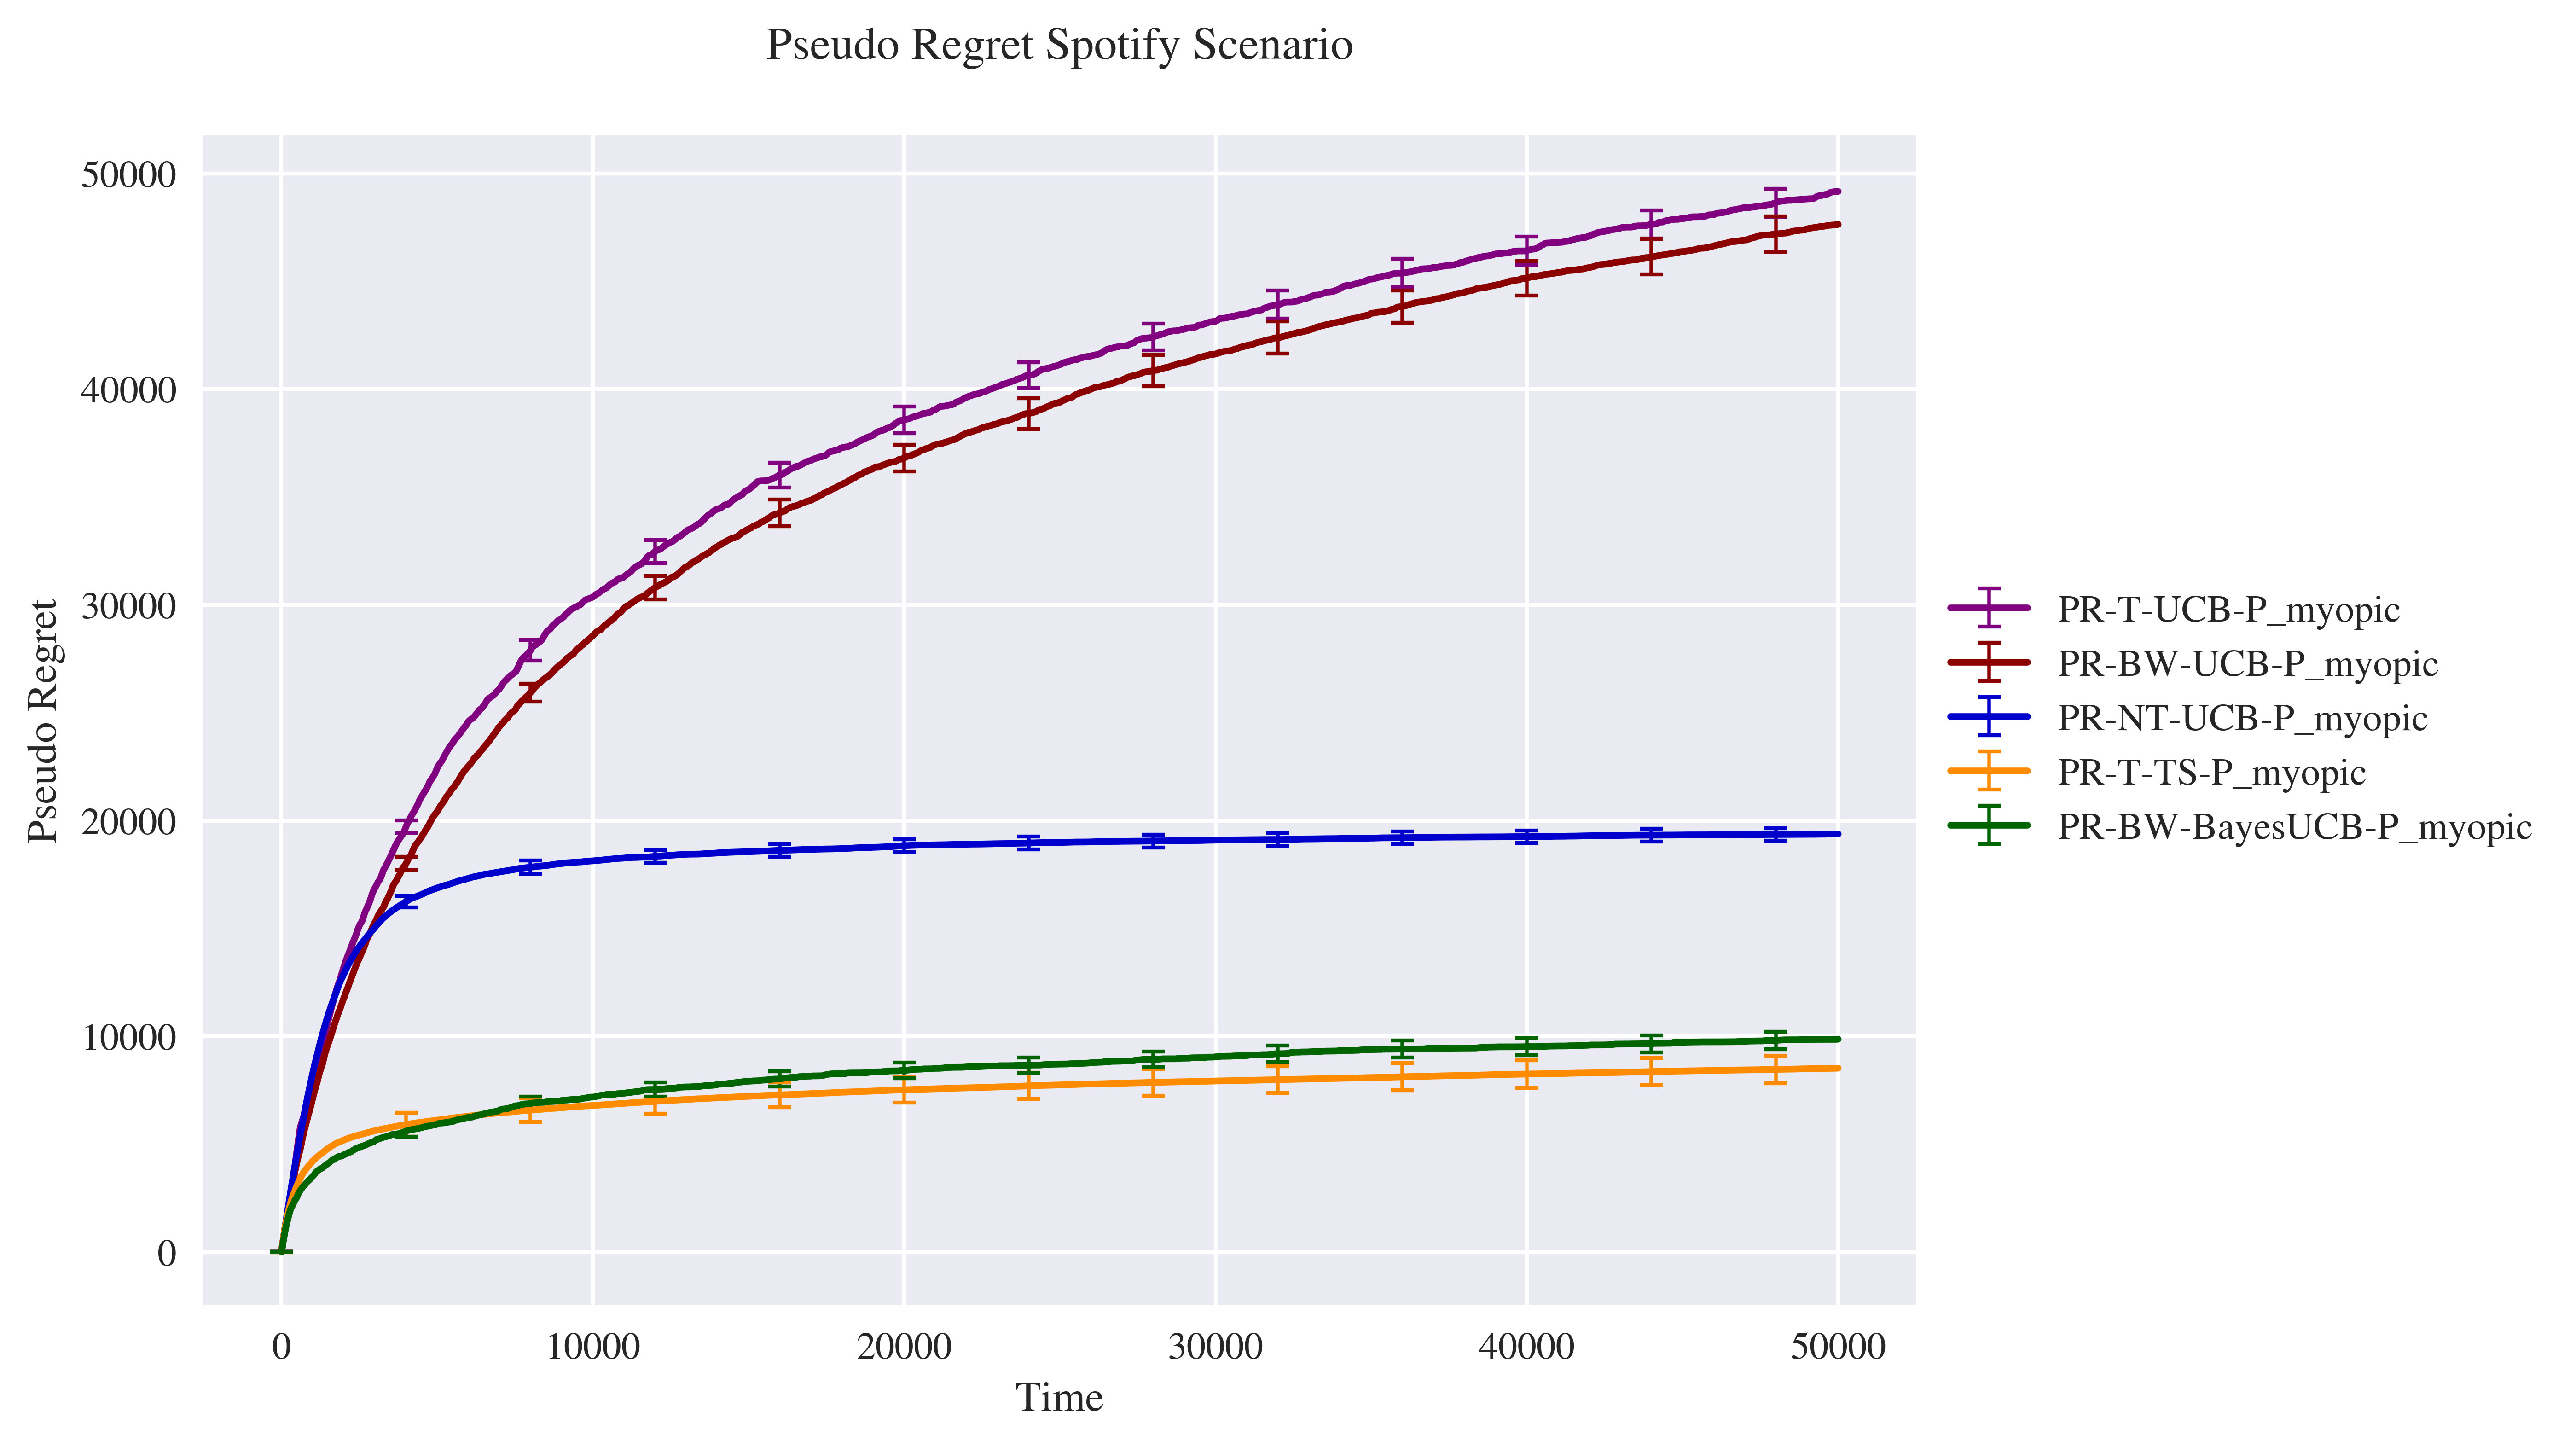
\includegraphics[width=16cm]{./images/ANALYTICS/experiment_spotify_def ANALYTICS.png}
		\centering	
		\caption{Pseudo regret plot of the experiment Spotify Playlist Problem.}
		\label{f:s}
\end{figure}




%RENT
\begin{figure}[H]
	\centering
	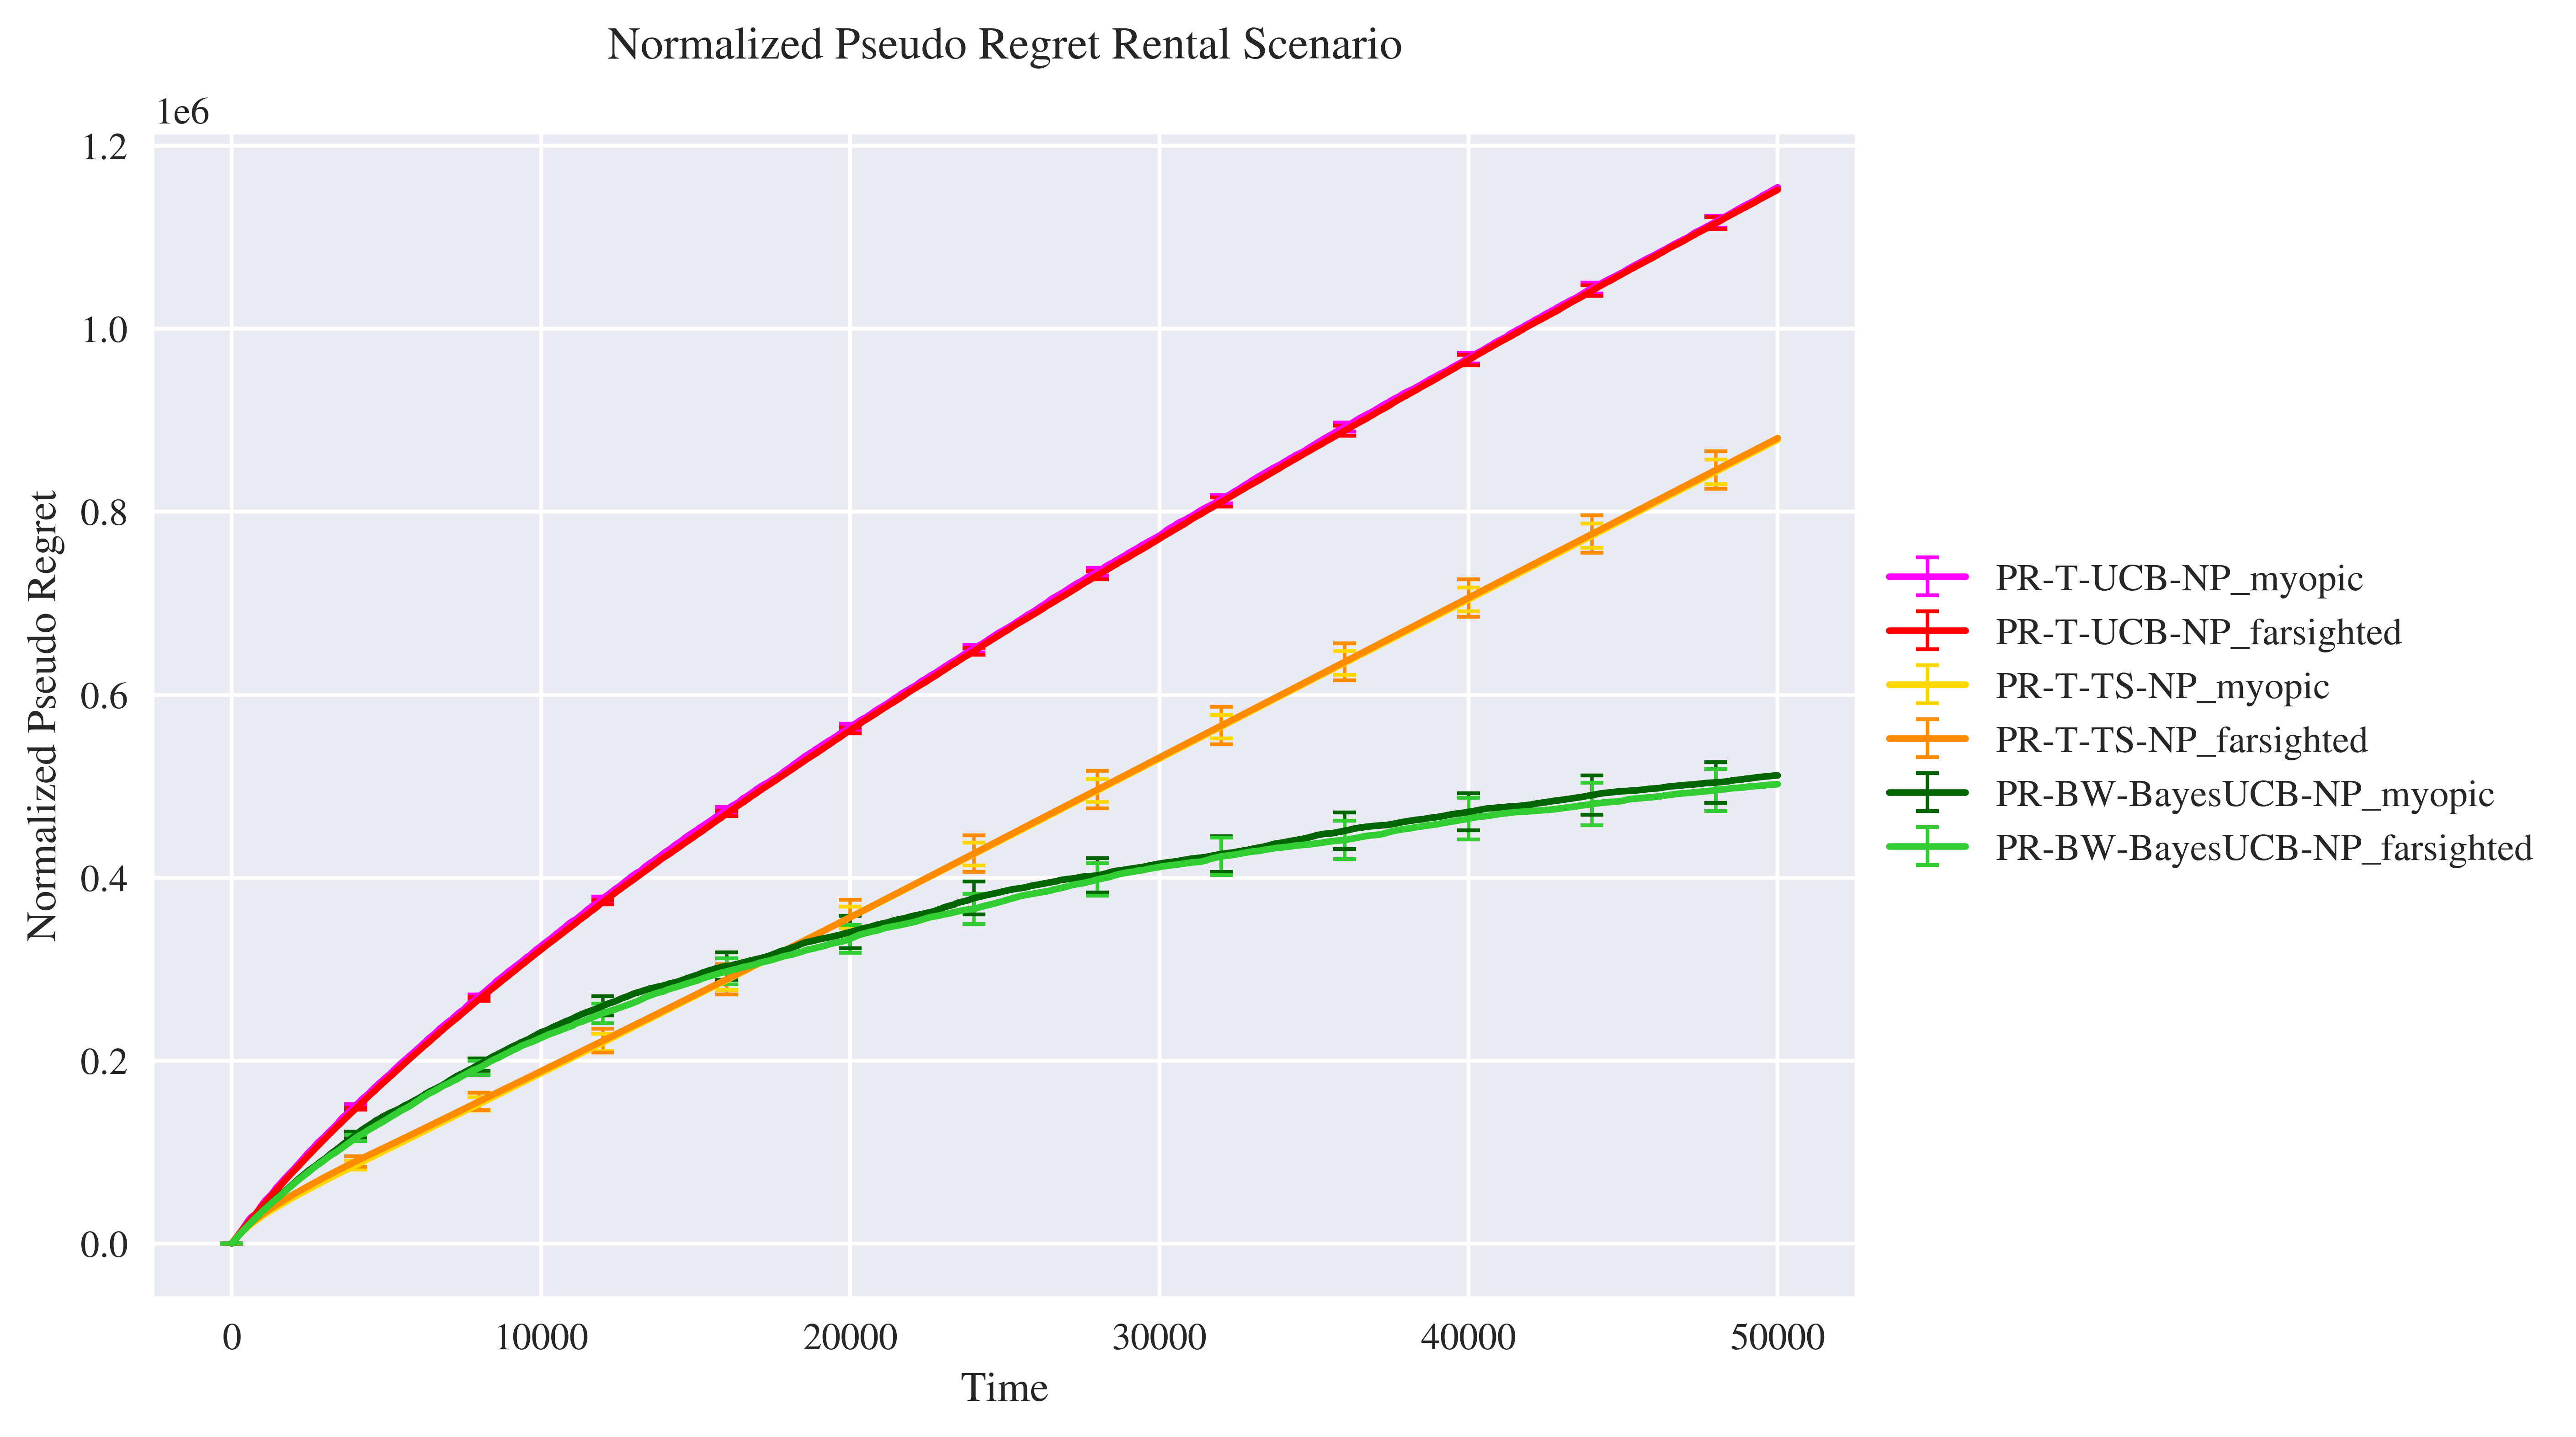
\includegraphics[width=16cm]{./images/ANALYTICS/affitti-def ANALYTICS.png}
		
	\caption{Normalized pseudo regret plot of the experiment Rental Pricing Problem.}
	\label{f:r}
\end{figure}




\section{Observations}
Empirical evidence shows that, in the majority of the addressed settings, the policies that adopt a Bayesian approach achieves better performance compared to ones that adopt the Frequentist approach.

In the settings Synthetic A and Synthetic B, respectively described in Sections \ref{SA} and \ref{SB}, the Frequentist algorithms which exploit partial information outperforms the Frequentist baselines. Also for the Bayesian algorithms, although less evident, the baselines have worse performance compared to the algorithms that exploit partial information. Settings Synthetic A and Synthetic B, despite having different characteristics, obtain the same algorithms ranking where PR-BW-BayesUCB-P is the best overall and PR-NT-UCB-P is the best among the Frequentist ones. 

The setting Synthetic C, described in Section \ref{SC}, shows an interesting situation. It results that the algorithm PR-NT-UCB-P suffers the magnitude of $\Tmax$ more than the other algorithms. In Figure \ref{f:c} we notice that, when $Tmax=50$, PR-NT-UCB-P is the best Frequentist algorithm, then, as $\Tmax$ increases, it performs worse than the others. For the other algorithms we have a result comparable to the one obtained in Synthetic A and Synthetic B.

All the synthetic settings presented are designed as an abstraction of possible real problems. For example the setting Synthetic B, could be seen as a simplified version of the Medical Trial problem proposed in Example \ref{trial}. The setting Synthetic C exemplifies the scenario of the dynamic pricing problem of a subscription-based service, behind the assumption that high prices discourage long persistency. In all the synthetic settings,  the best algorithm is the Bayesian PR-BW-BayesUCB-P, which exploits partial information during the reward acquisition process.

The experimental results show that an algorithm in farsighted configuration performs better than the same in myopic configuration. This is what we expected intuitively since the farsighted configuration anticipates information to the learner. However, this improvement is clearly noticeable only in a few cases, for example: PR-T-UCB-P in Figure \ref{f:a}, PR-BW-BayesUCB-P in Figure \ref{f:c} with $\Tmax=200$. This distinction is not relevant for the performance analysis of the algorithms.

While the synthetic settings analyzed are in tight-persistency, the Spotify Playlist problem described in Section \ref{spotify} is in general-persistency. The results of the Spotify experiment in Figure \ref{f:s} depict a different situation from the synthetic ones. In the Frequentist algorithms PR-BW-UCB-P is really close to the baseline PR-T-UCB-P and, in the Bayesian ones, the baseline PR-T-TS-P overtakes PR-BW-BayesUCB-P. This result leads us to think that the bin-wise approach suffers the general-persistency. As a matter of facts, while in the synthetic settings the reward is concentrated at the start of the buckets as depicted in Figure \ref{sbucket}, in this scenario the reward is uniformly distributed over the bucket. This nullifies the advantage of the bin-wise approach. The algorithm PR-NT-UCB-P, which exploit the non terminated buckets filling them with fake realizations, does not suffer the issue of the reward distribution along the bucket and outperforms both the baseline PR-T-UCB-P and the bin-wise Frequentist algorithm PR-BW-UCB-P.

The Rental Pricing problem described in Section \ref{rental}, appears more difficult than the other settings. Both the Frequentist and Bayesian baselines are not able to identify the best arm quickly, since they do not curve in the normalized pseudo-regret plot (Figure \ref{f:r}). Although the difficulty of the proposed scenario, the algorithm PR-BW-BayesUCB-NP outperforms the other ones.


